%&../.preamble
\endofdump
\usepackage{subcaption}
\usepackage{multirow}
\usepackage{circuitikz}
\title{Fondamenti matematici per l'informatica}
\author{Mattia Marini}

\begin{document}

\maketitle
\tableofcontents
\listofdefs
\listoftheorems
\section{Insiemistica}
\subsubsection*{Definzioni di base sugli insiemi}
\definizione{Insieme}{
	Un insieme è una \underline{collezione di oggetti}, detti suoi elementi. La caratteristica fondamentale di un insieme è che si possa stabilire senza ambguità se qualcosa vi appartiene o meno:
	\[
		x \in  A \text{ oppure } x \not \in A
	\]
}
Quest'ultima caratteristica, sembra scontata ma non lo è. Considera il seguente insieme:
\[
	A = \left\{x | x \not  \in  x \right\}
\]
Questo caso è noto come il \underline{paradosso di Russel}. $ A $ non può essere un insieme in quanto:
\begin{itemize}
	\item Se $ A \in A $ allora per definizione di $ A $, $ A \not  \in  A $
	\item Se $ A \not  \in  A $ allora per definizione di $ A $ , $ A \in  A $
\end{itemize}
\definizione{Insiemi uguali}{
	Due insiemi sono uguali se e solo se contengono gli stessi elementi. Formalmente
	\[
		A = B \Leftrightarrow \left(x \in  A \Leftrightarrow x \in B \; \forall x\right)
	\]
}
\definizione{Insieme vuoto}{
	E' costituito dall'insieme senza alcun elemento e denotato con il simbolo $ \emptyset  $. Formalmente un insieme è vuoto se
	\[
		x \not  \in A \; \forall x
	\]
}
\definizione{Insieme contenuto}{
	Si dice che $ A $ è \underline{contenuto} in $ B $ ($ A \subseteq B $) se:
	\[
		\left(x \in A \Rightarrow x \in B\right) \; \forall x
	\]
	Si dice che $ A  $ è \underline{contenuto strettamente} in $ B $ ($ A \subsetneq B  $) se:
	\[
		\left(x \in A \Rightarrow x \in B\right) \; \forall x \text{ e } A \neq B
	\]
}

\definizione{Definire degli insiemi}{
	Abbiamo principalmente due modi di definizre degli insiemi:
	\begin{itemize}
		\item  \textit{Proprietà:}   Se $ X $ è un insieme e $ P\left(x\right)  $ è una proprietà esprimibile sull'elemento $ x \in X $ allora il seguente è un insieme:
		      \[
			      \left\{x | x \in X \text{ e }P\left(x\right)\right\}
		      \]
		\item  \textit{Per elenco:} possiamo elencare uno per uno gli elementi dell'insieme stesso. Questa procedura può essere vista come un iterazione sugli elementi che andranno contenuti nell'insieme stesso
		      \[
			      \left\{1,2,3,\ldots ,n\right\}
		      \]
	\end{itemize}
}
\definizione{Operazioni su insiemi}{
	Se $X$ e $Y$ sono insiemi si costruiscono altri insiemi:
	\begin{itemize}
		\item \textit{Intersezione} $X \cap Y=\{x \mid x \in X$ e $x \in Y\}$
		\item \textit{Differenza} $X \backslash Y=\{x \mid x \in X$ e $x \notin Y\}$.
		      Quando $Y \subseteq X$ la differenza $X \backslash Y$ viene chiamata il complemento di $Y$ in $X$ e viene denotata anche con $\complement_X Y$ o semplicemente con $\complement Y$ o con $Y^{\prime}$ quando non ci sia ambiguità
		\item \textit{Unione} $X \cup Y=\{x \mid x \in X$ o $x \in Y\}$
		\item \textit{Differenza simmetrica} $X \triangle Y=(X \backslash Y) \cup(Y \backslash X)$
		\item \textit{Prodotto} $X \times Y=\{(x, y) \mid x \in X$ e $y \in Y\}$
		\item \textit{Potenza} $2^X=\{x \mid x \subseteq X\}$, ossia l'insieme contenente ogni sottoinsieme
	\end{itemize}
	Se $I$ è un insieme e per ogni $i \in I$ è dato un insieme $X_i$, si definiscono
	\begin{itemize}
		\item \textit{Intersezione} $\bigcap_{i \in I} X_i=\left\{x \mid \forall i x \in X_i\right\}$
		\item \textit{Unione} $\bigcup_{i \in I} X_i=\left\{x \mid \exists i x \in X_i\right\}$
	\end{itemize}
}
\subsection{Relazioni e funzioni fra insiemi}
\definizione{Relazione}{
	Siano $X$ e $Y$ insiemi si dice relazione tra $X$ e $Y$, un sottinsieme $\mathcal{R} \subseteq X \times Y$. Se $\mathcal{R}$ è una relazione si scriverà anche $x \mathcal{R} y$. Una relazione $\operatorname{tra} X$ e se stesso, si dirà anche una \textit{relazione binaria} su $X$.
}
\definizione{Funzione parziale}{
Una relazione $f \subseteq X \times Y$ si dice una \underline{funzione parziale} se per ogni $x \in X$ esiste al più un $y \in Y$ tale che $(x, y) \in f$. In simboli:
\[
	\forall x \in X\left((x, y) \in f \mathrm{e}\left(x, y^{\prime}\right) \in f\right) \Longrightarrow y=y^{\prime}
\]
Si scriverà $f: X \rightharpoonup Y$ per dire che $f$ è una funzione parziale da $X$ a $Y$ e in tal caso si scriverà anche $y=f(x)$ come sinonimo di $(x, y) \in f$.
}

\definizione{Dominio e immagine}{
	\textit{Dominio:} L'insieme $\{x \in X \mid \exists y \in Y: y=f(x)\}$ è detto il dominio di $f$ e si denota con $\operatorname{dom}(f)$
	\vskip3mm
	\textit{Immagine:} L'insieme $\{y \in Y \mid \exists x \in \operatorname{dom}(f): y=f(x)\}$ è detto l'immagine di $f$ e si denota con $\operatorname{im}(f)$.
}

\definizione{Funzione totale}{
	Una funzione parziale $f: X \rightarrow Y$ si dice funzione totale o semplicemente funzione se $\operatorname{dom}(f)=X$, in tal caso si scrive
	\[
		f: X \rightarrow Y
	\]
	Si denota $Y^X$ l'insieme di tutte le funzioni (totali) da $X$ a $Y$, ossia $Y^X=\{f$ : $X \rightarrow Y\}$
}
\definizione{Iniettività, surgettività e bigettività}{
	Una funzione $f: X \rightarrow Y$ si dice:
	\begin{itemize}
		\item \textit{iniettiva} se per ogni $x_1, x_2 \in X x_1 \neq x_2 \Rightarrow f\left(x_1\right) \neq f\left(x_2\right)$
		\item \textit{surgettiva} se per ogni $y \in Y$ esiste $x \in X$ tale che $f(x)=y$
		\item \textit{bigettiva} se è iniettiva e bigettiva
	\end{itemize}
}
\definizione{Funzione inversa}{
	Sia $f: X \rightarrow Y$ una bigezione, allora esiste un'unica funzione $g: Y \rightarrow X$ tale che $f \circ g=\mathrm{id}_Y$ e $g \circ f=\mathrm{id}_X$. Tale funzione si chiama inversa $d i$ $f e$ si denota con $f^{-1}$.
}
\subsection{Insiemi euipotenti}
\definizione{Insiemi equipotenti}{
	Siano $ x $ e $ y $ due insiemi. Si dice che $ x $ è \underline{equipotente} a $ Y $ oppure $ X $ ha la \underline{stessa cardinalità} di $ Y $ se
	\[
		\exists f: x \to y \text{ t.c. } f \text{ bigezione }
	\]
	se due insiemi sono equipotenti si scrive informalmente che $ X ~ Y $
}
\label{equipotenza}
Nota bene, vale che dati tre insiemi $ X, Y $ e $ Z $
\begin{itemize}
	\item $X$ è equipotente a se stesso.
	\item se $X$ è equipotente a $Y$ allora $Y$ è equipotente a $X$
	\item se $X$ è equipotente a $Y$ e $Y$ è equipotente a $Z$, allora $X$ è equipotente a $Z$.
\end{itemize}
\subsubsection{Equipotenza e numero di elementi}
Cerchiamo di colegare la nozioni che due insiemi \underline{equipotenti} hanno \underline{lo stesso numero di elementi}
\begin{itemize}
	\item Un insieme equipotente garantisce l'esistenza di una funzione $ f $ \underline{biettiva}
	\item Se $ f $ è \underline{iniettiva} allora ogni elemento ha una mappatura 1:1 con un elemento dell'insieme di arrivo
	\item Se $ f $ è \underline{surgettiva} allora ogni elemento dell'insieme d'arrivo viene collegato all'insieme di inizio tramite $ f $
	\item I due insiemi hanno necessariamente \underline{lo stesso numero di elementi}
\end{itemize}
\teorema{Cardinalità e equipotenza}{
	Dati due insiemi $ X $ e $ Y $, questi sono equipotenti se e solo se la loro cardinalità è la stessa
	\[
		X \sim Y \Leftrightarrow \left|X\right|=\left|Y\right|
	\]
}
\section{Costruzione dei numeri naturali}
\subsection{Assiomi di Peano}
Affrontiamo l'approccio assiomatico di Peano. Vediamo 4 assiomi:
\begin{itemize}
	\item L'insieme $ \N  $ contiene almeno un elemento $ 0 \in \N  $ (0 è detto \underline{zero})
	\item Esiste una funzione successivo $ succ: \N  \to \N  $ \underline{iniettiva}
	\item La funzione $ succ $ ha la seguente proprietà: $ succ\left(n \right) \subset \N \setminus \left\{0\right\} \; \forall  n \in  \N $
	\item \underline{Assioma di induzione}. Sia $ A $ un sottoinsieme di $ \N  $. Supponiamo che $ A $ soddisfi le seguenti due proprietà:
	      \begin{itemize}
		      \item (\textit{Base dell'induzione}) $ 0 \in A $
		      \item (\textit{Passo induttivo}) $  \forall n \in  \N \left(n \in A\right) \Rightarrow succ\left(n\right) \in A $
	      \end{itemize}
	      Allora $ A = \N  $
\end{itemize}
Inoltre ho proprietà importanti:
\begin{itemize}
	\item Siam $ n \in  \N \setminus \left\{0\right\}$ allora  $\exists ! n \in  \N \text{ t.c. } succ\left(m\right) = n $. In questo caso $ n  $ è detto predecessore di $ m $
	      \begin{itemize}
		      \item Visto che $ succ\left(n\right) $ è una funzione iniettiva, se esiste, il predecessore deve essere unico
		      \item Procediamo poi \underline{per assurdo} ammettendo che esista un $ n $ che \underline{non} abbia predecessore
		            \begin{itemize}
			            \item Supponiamo che esista un $ m \neq 0$ che non abbia predecessore, ossia $ succ\left(n\right) \neq m \; \forall n \in \N  $
			            \item Creo insieme $ A $ senza $ m $: \[
				                  A = \N \setminus \left\{m\right\}
			                  \]
			            \item Chiaramente $ 0 \in A $ in quanto $ m \neq 0 $
			            \item Chiaramente $ succ \left(n\right) \in A $ in quanto per definizione $ A = \N  \setminus \left\{m\right\}$
			            \item Per l'assioma di induzione quindi $ A = \N  $. Questa è tuttavia una \underline{contraddizione}
		            \end{itemize}
	      \end{itemize}
\end{itemize}
\teorema{Principio di induzione di prima forma}{
	Sia $ \left\{P\left(n\right)_{n \in \N }\right\} $ una famiglia di proposizioni (affermazioni) $ P\left(n\right) $ indicizzata su $  n \in  \N  $ sulla quale valgono le seguenti proprietà:
	\begin{itemize}
		\item \textit{(Base dell'induzione)} $ P\left(0\right) $ è vera
		\item \textit{(Ipotesi induttiva)} $  \forall n \in  \N :\left[P\left(n\right) \Rightarrow P\left(succ\left(n\right)\right)\right] $ ossia se $ P\left(n\right) $ è vera allora anche $ P\left(succ\left(N\right)\right) $ è vera.
	\end{itemize}
	Allora $ P\left(n\right) $ è vera $  \forall n \in  \N $
}
Dimostrazione:
\begin{itemize}
	\item Sia $ A = \left\{n \in  \N | P\left(n\right) \text{ è vera }\right\} $
	\item Sappiamo che
	      \begin{itemize}
		      \item $ 0 \in  A $ (base dell'induzione)
		      \item se $ n \in  A $ allora $ succ\left(n\right) \in A $ quindi $  A = \N  $
	      \end{itemize}
\end{itemize}
Ho quindi esteso la proprietà ad ogni $ n \in  \N  $ per gli assiomi di Peano
\teorema{Teorema di ricorsione}{
	Sia $ X $ un insieme \underline{non vuoto}, sia $ h:\N_{x}X \to X $ una funzione (mappa) e sia $ c \in  X$. $ c $ è detto \underline{dato iniziale}, $ h $ \underline{funzione di iterazione}. Allora $  \exists ! f: \N  \to x  $ tale che:
	\[
		\begin{cases}
			f\left(0\right)=c                                                                            \\
			\forall  n \in  \N \quad f\left(succ\left(n\right)\right) = h\left(n, f\left(n\right)\right) \\
		\end{cases}
	\]
}
\subsubsection*{Applicazioni del teorema di ricorsione}
Sia $ m \in  \N  $. Vogliamo formalizzare il concetto di \underline{somma a sinistra con $ m $}.
\begin{itemize}
	\item Sia $ x = \N  $, sia $  c = m $ e sia $ h : \N  x \N  \to \N  $ definita ponendo $ h\left(a,b\right):= succ\left(b\right) $.
	\item Allora grazie al teorema di ricorsione $  \exists ! f: \N  \to x = \N  $ tale che :
	      \[
		      \begin{cases}
			      f\left(0\right)=c                                                                            \\
			      \forall  n \in  \N \quad f\left(succ\left(n\right)\right) = h\left(n, f\left(n\right)\right) \\
		      \end{cases}
	      \]
	      $ f $ è detta \underline{somma a sinistra} con $ m $
\end{itemize}
\subsection{Ordinamento di un insieme}
Una volta definiza l'addizione su $ \N  $ si può definire anche l'operatore $ \le  $:
\definizione{Operatore minore uguale}{
	Siano $ n,m \in \N  $. Diremo che $ n \le m $ se esiste un $ k $ tale che
	\[
		n + k = m
	\]
}
Si può vedere $\leq$ come un sottinsieme di $\mathbb{N} \times \mathbb{N}$ e precisamente
\[
	\leq=\{(n, m) \in \mathbb{N} \times \mathbb{N} \mid \exists k \in \mathbb{N}: n+k=m\}
\]
E quindi $\leq$ è una relazione (definizione 1.9) sui naturali e quello che abbiamo definito come significato di $n \leq m$ è effettivamente lo stesso che dire $(n, m) \in \leq$.
\definizione{Ordinamento di un insieme}{
	Sia $ X $ un insieme non vuoto e sia $ \le $ una \underline{relazione binaria}. $ \le $ si dice ordinamento parziale di $ X $ se:
	\begin{enumerate}
		\item \textit{Riflessiva} $ x \le x  \;\forall  x \in  X$
		\item \textit{Antisimmetrica} $  \forall x,y \in X:\left(x \le y\right) $ e $ \left(y \le x\right) \Rightarrow  x = y $
		\item \textit{Transitiva} $  \forall  x,y,z \in  X: \left(x \le y\right) \text{ e } \left(y \le z\right) \Rightarrow  \left(x \le z\right) $
	\end{enumerate}
	la relazione $ \le  $ si dice \underline{ordinamento parziale} di un insieme. Inoltre se:
	\begin{enumerate}\setcounter{enumi}{3}
		\item \textit{Tricotomia} $  \forall x,y \in X, \left(x \le y\right) $ oppure $ \left(y \le x\right) $
	\end{enumerate}
}

Nota che è semplice dimostrare che $ \N  $ è un insieme \underline{parzialmente ordinato}. Tuttavia dimostrare che è un insieme \underline{totalmente ordinato} è un procedimento piuttosto tedioso.
\teorema{Principio di induzione shiftato di prima forma}{
Sia $ \left\{P\left(m\right)\right\}_{m \ge k} $ una famiglia di proposizioni (affermazioni) indicizzate seui numeri naturali $ \ge $ di un certo $ k \in  \N  $ fissato. Supponiamo che:
\begin{itemize}
	\item \textit{Base induzione} P(k) è vera
	\item  \textit{Passo induttivo} $  \forall  n \in  \N , n \ge k : \left(p\left(n\right) \Rightarrow P\left(n+1\right)\right) $
\end{itemize}
}
\section{Esercizi per induzione}
\subsubsection*{Esercizio 2}
Dimostra che
\begin{equation}\label{esinduzione2}
	\sum_{k=1}^{n} 6k ^2 = n\left(n+1\right)\left(2n+1\right)
\end{equation}
\begin{itemize}
	\item \textit{Passo base.} Per $ n = 2 $ chiaramente vale:
	      \[
		      \sum_{k=1}^{2} 6k^2 = \left(6\cdot 1^2\right)\left(6\cdot 2^2\right) = 6 + 24 = 30
	      \]
	      e anche
	      \[
		      2 \left( 2+1\right)\left(2 \cdot 2 + 1\right) = 30
	      \]
	\item  \textit{Passo iduttivo}. Assumo che l'equazione \ref{esinduzione2} sia vera per $ n \ge 2 $.
	\item
	      \begin{align*}
		      \sum_{k=1}^{n+1} 6k^2 & = \sum_{k=1}^{n} 6k^2 + 6\left(n+1\right)^2                                                                                                   \\
		                            & = n\left(n+1\right)\left(2n+1\right) + 6 \left(n+1\right)^2= \left(n+1\right) \left(\left(n+1\right)+1\right)\left(2\left(n+1\right)+1\right)
	      \end{align*}
\end{itemize}
\subsection{Cardinalità su insiemi finiti}
Per ogni $ n \in  \N  $, indichiamo con $ I_{n} $ il seguente sottoinsieme di $ \N  $:
\[
	I_{n} = \left\{0,1,\ldots , n-1\right\}
\]
Inoltre poniamo $ I_0= \emptyset  $
\definizione{Insieme finito}{
	Dato un insieme $ X $, diciamo che $ X $ \underline{è finito} se esiste un n tale che $ X $ è \underline{equipotente} a $ I_n $:
	\[
		\exists n \in \N \text{ t.c. } X \sim I_n
	\]
	se $ X $ non è finito si dice \underline{infinito}
}
tuttavia può sorgere il dubbio se $ X $ è equipotente con solo un $ I_n $ oppure con molteplici $ I_n $. Per risolvere questo dubbio serve il \underline{teorema dei cassetti}
\teorema{Teorema dei cassetti}{
	Siano $ X $ e $ Y $ insimemi e siano $ n,m \in  \N  $ tali che:
	\begin{itemize}
		\item $ n < m $
		\item $ X \sim I_n $
		\item $ Y \sim I_m $
	\end{itemize}
	Allora \underline{non} esiste alcuna funzione $ f: y \to x $ \underline{iniettiva} (y ha più elementi)
}
\label{teo:cassetti}
La dimostrazione procede per induzione, indicizzando $ n \in \N  $. L'ipotesi induttiva va fatta sulla $ n $: fissata una $ n $, la $ m $ può essere qualsiasi numero naturale maggiore di $ n $
\begin{itemize}
	\item \textit{Passo base con $ P\left(0\right) $}:
	      \begin{itemize}
		      \item $  n = 0, m > 0 $
		      \item $ X \sim I_0 \sim \emptyset $
		      \item Tuttavia abbiamo dimostrato che \underline{non} eisiste alcuna funzione $ f: Y \to X $ che va da un insieme non vuoto ad un insieme $ X = \left\{\emptyset\right\} $
	      \end{itemize}
	      Ho quindi dimostrato  che la proprietà è verificata su $ P\left(0\right) $
	\item Assumiamo che l'ipotesi sia verificata per $ n $, e dimostriamo che allora lo deve essere anche per $ n+1 $. Per fare ciò procediamo per assurdo, supponendo che esista $ f:Y \to X  $ iniettiva
	      \begin{itemize}
		      \item L'insieme $ X $ è in bigezione con $ I_{n+1} $
		      \item Supponiamo di togliere da $ X $ l'elemento collegato dalla bigezione $ g $ fra $ X $ e $ I_n $
		      \item $ g\left(n\right) \not\in f\left(y\right) $
		            \begin{itemize}
			            \item
			                  i
		            \end{itemize}
		      \item $ g\left(n\right) \not\in f\left(y\right) $
		            \begin{itemize}
			            \item Poichè $ f $ è iniettiva, $ f^{-1}\left(x_n\right) $ sarà un singolo elemento
			            \item Posso rimuovere dunque sia $ x_n $ che $ f^{-1}\left(x_n\right) $. Chiamo questi nuovi due insiemi $ X' $ e $ Y' $
			            \item Posso considerare $ f: Y' \to X' $. $ f $ è sempre iniettiva
			            \item Questo è tuttavia impossibile in quanto per \underline{ipotesi} induttiva è stato supposto che per $ n \quad \not\exists f: Y \to X $ iniettiva
		            \end{itemize}
	      \end{itemize}
\end{itemize}
Posso rinforzare questa affermazione con il seguente corollario:
\teorema{Colorrario a teorema dei cassetti}{
	Siano $ X $ e $ Y $ due insiemi e siano $  n, m \in \N  $ tali che $  x \sim I_n  $ e $ Y \sim I_m $, allora:
	\[
		X \sim Y \Leftrightarrow n = m
	\]
}
\textbf{Dimostrazione}
\begin{itemize}
	\item $ \Leftrightarrow $Se $ n=m $ allora $ X \sim Y $ per composizione di \underline{bigezioni}
	\item Se $ X \sim Y $ e $ X \sim I_n, Y \sim I_m $, allora $ I_n \sim I_m $
	\item Per il lemma dei cassetti, non può esistere una iniezione fra $ I_m $ e $ I_n $ se $ n \neq m $. Quindi se esiste una bigezione fra questi, devono avere lo stesso numero di elementi
\end{itemize}
\definizione{Cardinalità}{
	Dato un insieme finito $ X $ si dice che la cardinalità di $ X $ è $ n $ se
	\[
		X \sim I_n
	\]
	si dice informalmente che $ \left|X\right|= n$, anche se il valore assoluto indicherebbe l'insieme cardinale. $ \left|X\right| = I_n $  sarebbe la notazione corretta
}
\teorema{}{
	Sia $ X $ un insieme finito e sia $ Y $ un suo sottoinsieme. Allora
	\[
		Y \text{ è un insieme \underline{finito} e } \left|Y\right| \le \left|X\right|
	\]
	Inoltre se $ Y \subset X $ allora $ \left|Y\right| < \left|X\right| $
}
\subsubsection*{Dimostrazione}Procedo per induzione indicizzando la cardinalità di $ X $.
\begin{itemize}
	\item  Per $ \left|X\right| = 0 $ è verificata in quanto $ \left|X\right| = I_0 = \emptyset $. L'unico sottoinsieme del vuoto è il vuoto e ha cardinalità 0
	\item Come in dimostrazione del teorema dei cassetti (\textit{teo \ref{teo:cassetti}})
\end{itemize}
Questo teorema ha un risvolto importantissimo, ossia che $ \N  $ è un insieme infinito.
\definizione{Buon ordinamento}{
	Sia $ X $ un insieme e sia $ \le  $ un ordinamento totale su $ X $. Se ogni sottoinsieme non vuoto $ A $ di $ X $ ammette minimo (rispetto al $ \le  $), allora $ \le  $ si dice \underline{buon ordinamento su $ X $}. In questo $ \left(X, \le \right) $ si dice \underline{insieme ben ordinato}
}
La caratteristica importante di un insieme ben ordinato è che vale su di esso un principio di induzione fortissimo: il principio di induzione di seconda forma.
\teorema{Buon ordinamento dei numeri naturali}{
	L'insieme dei numeri naturali dotato dell'ordinamento $ \le  $ standard, ovvero la coppia $ \left(\N , \le \right) $, è \underline{ben ordinato}
}
\subsubsection*{Dimostrazionie}
Sia $  A $ un sottoinsiieme di $ \N  $ \underline{senza minimo}. Dobbiamo provare che $ A = \emptyset  $
\begin{itemize}
	\item Dimostriamo per induzione che per ogni $ n \in  \N  $ vale:
	      \[
		      \left\{0,1,\ldots ,n\right\} \subset B : = \N  \setminus A
	      \]
	\item
	      i
\end{itemize}
\hypertarget{diveuclidea}{\subsection{La divisione euclidea} }
Assumiamo la conoscenza dell'insieme $ \Z = \left\{\ldots -2,-1, 0 ,1,2,\ldots ,n,\ldots \right\} $
\teorema{Esistenza ed unicità della divisione euclidea}{
	Siano $ n $ ed $ m $ tale che $ m \neq 0$. Allora esistono e sono \underline{unici} due interi $ q, r \in \Z $ tali che
	\[
		\begin{cases}
			n = q m + r \\
			0 \le  r \le  \left|m\right|
		\end{cases}
	\]
	inoltre se $ n, m \in \N  $, $ m > 0 $ allora $ q,r \in  \N  $
}\label{divisioneeuclidea}
\subsubsection*{Dimostrazione esistenza}
Fisso come parametro $ m > 0$ e procediamo con il principio di induzione di seconda forma, usando come ipotesi induttiva che
\[
	P\left(n\right)= \left(\exists q,r \in  \N  \text{ t.c. } \begin{cases}
		n = qm + r \\ 0 \le  r < m
	\end{cases}\right)
\]
\begin{itemize}
	\item \textit{Passo base} La $ P\left(0\right) $ è vera con $ q = r = 0 $
	\item \textit{Passo induttivo} Assumiano di essere in grado di saper effettuare la divisione euclidea di $ k $ per $ m $ per ogni $ k < n $ (ossia avere l'esistenza e unicità di $ q,r $). Se dimostro che ciò è possibili anche per $ n $ ho finito. Considero 4 casi:
	      \begin{align*}
		       & n > 0, m > 0 & n > 0, m < 0  \\
		       & n < 0, m > 0 & n < 0 , m < 0
	      \end{align*}
	\item $ n > 0, m > 0 $
	      \begin{itemize}
		      \item Se $ m > n $ allora basta prendere $ q = 0 $ e $ r = n $
		      \item Se $ n > m $ allora posso considerare la divisione fra $ n - m $ e $ m $. Questa divisione esiste per ipotesi induttiva la divisione euclidea esiste $ \forall k < n $ (chiaramente $ n-m < n $, visto che $ m > 0 $). Allora :
		            \[
			            \begin{cases}
				            n-m = qm + r \\
				            0 \le r < m
			            \end{cases}
		            \]
		            da cui la prima è uguale a
		            \[
			            n = m + qm + r = \left(q + 1\right)m + r
		            \]
		            Se ci pensi ha senso. $ m $ sta in $ n $ una volta in più $ \left(q+1\right) $
	      \end{itemize}
	\item $ n < 0, m > 0 $
	      \begin{itemize}
		      \item Visto che $ n < 0 $, per quanto dimostrato fin'ora, vale che:
		            \[
			            -n = mq + r \Rightarrow n = m \left(-q\right) -r
		            \]
		      \item Se $ r =0 $ ho finito. Altrimenti agggiungendo e sottraendo $ m $ ottengo
		            \[
			            n = m \left(-q\right) - m - r + m = \left(-q - 1\right)m + m - r
		            \]
		      \item Visto che per definizione $ 0 < r < m $, allora vale che $ 0 < m - r < m $
	      \end{itemize}
	\item $ n > 0, m < 0 $
	      \begin{itemize}
		      \item Come nel caso precedente, moltiplico per -1 e mi baso su quanto già dimostrato
	      \end{itemize}
	\item $ n < 0, m < 0 $
	      \begin{itemize}
		      \item Come nel caso precedente, moltiplico per -1 e mi baso su quanto già dimostrato
	      \end{itemize}
\end{itemize}
\subsubsection*{Dimostrazione unicità}
Supponiamo per assurdo $ q $ ed $ r $ non siano unici. Avrei:
\[
	\begin{cases}
		n = qm + r \\
		0 \le  r < \left|m\right|
	\end{cases}
	\quad
	\text{e}
	\quad
	\begin{cases}
		n = q'm + r' \\
		0 \le  r < \left|m\right|
	\end{cases}
\]
quindi avrò che
\[
	qm + r = q'm + r' \rightarrow qm -q'm = r' - r \rightarrow \left(q- q'\right)m = r' - r
\]
visto che la differenza di resti deve necessariamente essere $ < \left|m\right| $ in quanto entrambi i resti sono per definizione valori \underline{positivi}, vale che:
\[
	\left|\left(q- q'\right)\right|\left|m\right| = \left|r' - r\right| < \left|m\right| \rightarrow \left|\left(q-q'\right)\right|< 1
\]
ma visto che $ \left|q - q'\right|< 1 $ e $ q $ e $ q' $ sono per def \underline{numeri interi}, allora $ q- q' =0$, ossia \underline{$ q = q' $}

\subsection{Scrittura dei numeri naturali in base maggiore di 2}
\definizione{Rappresentazione numeri naturali}{
	Sia $  b \in  \N  $. Diremo che un numero naturale $ n \in  \N  $ è \underline{rappresentabile in base $ b $} se esistono $ k \in  \N  $ $ \varepsilon_0, \varepsilon_1,\ldots , \varepsilon_k $ tali che :
	\begin{itemize}
		\item $ \varepsilon_0, \varepsilon_1,\ldots , \varepsilon_k  \in  I_b $, dove $ I_b = \emptyset  $ se $ b = 0 $, $ I_b = \left\{0,1,\ldots ,b-1\right\} \text{ se } b \ge 1$
		\item $ n = \varepsilon_0 b^{0}+ \varepsilon _1b^{1}+ \varepsilon_2 b^{2}+ \ldots + \varepsilon_k b^{k}  = \sum_{i=0}^{k} \varepsilon _i b^{i}$
	\end{itemize}
	In questo caso $ \varepsilon_0, \ldots , \varepsilon_k $ si dicono \underline{cifre} di $ n $ in base $ b $ e si scrive:
	\[
		n = \left(\varepsilon_0,\ldots ,\varepsilon _k\right)_b
	\]
}
\label{rappnumnat}
Nota che
\begin{itemize}
	\item In base $ 0 $ non è rappresentabile nulla in quanto :
	      \[
		      I_0 = \emptyset
	      \]
	\item In base 1 è rappresentabile solo lo 0 in quanto :
	      \[
		      I_1 = \left\{0\right\}
	      \]
\end{itemize}
\hypertarget{teorappnum}{}
\teorema{Rappresentabilità dei naturali in base $ b $}{
Sia $ b \ge 2 $. Allora per ogni $ n \in  \N  $ esiste una succesione $ \left\{\varepsilon _i\right\}_{i \in  \N } $ tale che soddisfi le proprietà enunciate in \ref{rappnumnat}
tale espressione è inoltre \underline{unica}
}
\subsubsection*{Dimosrazione esistenza}
Procedo per induzione su $ n $:
\begin{itemize}
	\item \textit{Passo base} Per $ n = 0 $ l'hp è verificata. Basta prendere una stringa di soli $ 0 $
	\item \textit{Passo induttivo di seconda forma} Prendo un $ n > 0 $ e assumo l'hp vera per ogni $ k < n $. Assumiano di saper quindi rappresentare ogni $ k $ in base $ b $ per ogni $ k < n $
	      \begin{itemize}
		      \item Eseguiamo la divisione di $ n  $ per $ b $:
		            \[
			            \begin{cases}
				            n = qb + r \\
				            0 \le  r < b \Leftrightarrow r \in  I_b = \left\{0,1,\ldots , b-1\right\}
			            \end{cases}
		            \]
		      \item Dimostro che $ q < n $
		            \begin{itemize}
			            \item se $ q = 0 $ è banalmente verificata
			            \item Se $ q \neq 0 $ allora so che $ q < qb $ in quanto $ b \ge 2 $. Allora anche $ q<qb + r = n $
		            \end{itemize}
		      \item Poichè $ q < n $ so che, per \textit{hp ind} $ q $ è rappresentabile in base $ b $, quindi
		            \[
			            n = qb + r = \left(\sum_{i = 0}^{\infty} \varepsilon_i b^{i}\right)b + r = \left(\sum_{i=0}^{\infty} \varepsilon _i b^{i+1}\right) + r
		            \]
		            \[
			            = \sum_{i = 1}^{\infty} \varepsilon_{i-1}b^{i} + r
		            \]
	      \end{itemize}
	      Nota che ciò che ottieni è un numero rappresentato secondo le proprietà elencate in \ref{rappnumnat}, in cui la $ \varepsilon_0 = r $ (nella sommatoria manca la cifra $ \varepsilon_0 b^{0} $)
\end{itemize}
\subsubsection*{Dimostrazione unicità}
Procedo per induzione su $ n $.
\begin{itemize}
	\item \textit{Passo base}. Per $ n = 0 $ l'unica rappresentazione ammessa è la stringa contenente soli zeri.
	\item \textit{Passo induttivo}. Suppongo che la rappresentazione sia unica $ \forall  k < n $
	      \begin{itemize}
		      \item Supponiamo per assurdo che esistano due rappresentazioni di $ n $ in base $ b $
		            \[
			            n = \sum_{i=0}^{\infty} \varepsilon_i b^{i} = \sum_{i=0}^{\infty} \varepsilon '_i b^{i}
		            \]
		      \item  Possiamo modificare le sommatorie estraendo il termine per $ i=0 $ e portando fuori un fattore $ b $
		            \[
			            n = b\sum_{i=1}^{\infty} \varepsilon_i b^{i-1} + \varepsilon _0= b\sum_{i=1}^{\infty} \varepsilon '_i b^{i-1} + \varepsilon' _0
		            \]
		      \item Nota che ho espresso $ n $ come divisione euclidea fra $ n $ e $ b $. Quindi per teo \ref{divisioneeuclidea} il resto è unico $ \varepsilon_0 = \varepsilon' _0 $. Allora stesso modo, $  q = \sum_{i=1}^{\infty} \varepsilon_i b^{i-1} = \sum_{i=1}^{\infty} \varepsilon'_i b^{i-1}$
		      \item Inoltre, come dimostrato precedentemente, $ q < n $, quindi per hp induttiva la rappresentazione è unica, ossia $ \varepsilon_i = \varepsilon'_i \quad \forall  i $
	      \end{itemize}
\end{itemize}
\section{Divisibilità}
\definizione{Divisibilità}{
	Siano $ n,m \in  \Z  $. Diciamo che \underline{$ n $ divide $ m $} e scriveremo $ n|m $ se
	\[
		\exists k \in  \Z \text{ t.c. } nk = m
	\]
	Se ciò è falso si dice che $ n $ non divivde $ m $ e si scrive $ n \not | m $
}
\begin{minipage}[t]{0.48\textwidth}
	Nota che valgono le seguenti proprietà:
	\begin{itemize}
		\item $ \forall n \in  \Z \rightarrow n | 0 $
		\item $ \forall  n \in \Z  \setminus \left\{ 0\right\} \rightarrow  0 \not | n $
		\item $ \forall  n \in \Z \rightarrow
			      \begin{cases}
				      \pm 1 | n \\
				      \pm n | n
			      \end{cases}$
	\end{itemize}
\end{minipage}
%
\begin{minipage}[t]{0.48\textwidth}
	Inoltre, se ho $ n,m,q \in \Z  $ vale che:
	\begin{itemize}
		\item $ n|m \text{ e } m|q \rightarrow n = \pm q $
		\item $ n|m \text{ e } m | n \Rightarrow  n = m \text{ oppure } n = -m $
	\end{itemize}
\end{minipage}
\definizione{Massimo comune divisore}{
	Siano $ n , m \in  \Z  $ \underline{non entrambi nulli}. Si dice che un numero $ d \in  \Z  $ è un \underline{massimo comune divisore}(M.C.D) tra $ m $ e $ n $ se
	\begin{itemize}
		\item $ d > 0 $
		\item $ d|n $ e $ d|m $
		\item Se $ c \in \Z  $ è tale che $ c|n $ e $ c|m $, allora $ c|d $
	\end{itemize}
}
Come mai non possono essere entrambi nulli? In quanto la famiglia dei divisori di entrambi i numeri sarebbe tutto $ \Z  $ (ogni numero divide 0)
\hypertarget{teomcd}{}
\teorema{Esistenza ed unicità M.C.D}{
	Siano $ n, m \in \Z  $ non entrambi nulli. Allora
	\[
		\exists! \left(n,m\right)
	\]
	ossia \underline{esiste ed è unico} l'M.C.D. fra $ n $ e $ m $
}
\subsubsection*{Dimostrazione esitenza}
Definiamo innanzitutto il seguente insieme $ S $ si $ \N  $:
\[
	S = \left\{s \in  \N  | s > 0, s = xn + ym\right\}
\]
per qualche $ x,y \in \Z $, ossia tutte le combinazioni lineari maggiori di zero fra $ n, m $. Nota che l'insieme è \underline{non vuoto} in quanto entrambi $ n,m $ sono non nulli:
\[
	x = n, y = m \rightarrow n^2  + m^2 > 0
\]
Poichè $ S $ è un sottoinsieme \underline{non vuoto} di $ \N  $, grazie al teorema del \underline{buon ordinamento}, allora ammete un minimo:
\[
	d = min\left(S\right)
\]
Poichè $ d \in  S $, vale :
\[
	\begin{cases}
		d > 0 \\
		\exists  x, y \in  \Z \text{ t.c. } d = xn + ym
	\end{cases}
\]
Nota che vale che ogni divisore comune fra $ n $ e $ m $ divide $ d $:
\begin{itemize}
	\item Dato $ c $ tale che $ c|n $ e $ c|m $, allora ho che $ n = kc, m = hc $
	      \[
		      d = xn + ym = xkc + yhc = c \left(xk + yh\right)
	      \]
\end{itemize}
Dimostriamo ora che $ d = xn + ym $ divide $ n $ e $ m $:
\begin{itemize}
	\item Considero la divisione euclidea tra $ n $ e $ d $:
	      \[
		      \begin{cases}
			      n = q\left(xn + ym\right) +r \\
			      0 \le  r < d = \left(xn + ym\right)
		      \end{cases}
	      \]
	\item Supponiamo per assurdo che $ r \neq 0 $, allora avrei:
	      \[
		      r = n-q\left(xn + ym\right) = n - qxn - qym = n \left(1 - qx\right) + m\left(-qy\right)
	      \]
	      quindi $ r \in  S $, ma per le caratteristiche del rest della divisione euclidea $ 0 \le  r < d $, ossia $ r < d = min\left(S\right) $, il che è un assurdo logico visto che $ r \in S $
\end{itemize}
Analogamente si dimostra che $ d | m $
\subsubsection*{Dimostrazione unicità}
Per definizione un numero è M.C.D. fra $ m,n $ se è divisibile per ogni divisore comune a $ n,m $
\begin{itemize}
    \item Siano $ d, d' $ due M.C.M. di $ n,m $
    \item Visto che $ d|n, d|m $, allora è un divisore comune, quindi $ d|d' $
      \item Al contrario, visto che $ d'|n, d'|m $, allora è un divisore comune, quindi $ d'|d $
\end{itemize}
Visto che $ d'|d $ e $ d | d' $ allora $ d = \pm d' $. Per definizione, il massimo comune divisore deve essere un intero positivo, quindi da questo deriva l'unicità
\teorema{Lemma utile}{
	Siano $ c,n,m \in  \Z  \text{ t.c. } c | n \text{ e } c | m  $. Per ogni $  x , y \in  \Z  $ si ha:
	\[
		c \vert (xn + ym)
	\]
}
\subsection{Criterio d'arresto}
L'M.C.D gode delle seguenti proprietà:
\begin{itemize}
	\item Non conta il segno (posso considerare il valore assoluto dei numeri)
	      \[
		      \left(n,m\right) = \left(-n,m\right) = \left(n, -m\right) = \left(-n,-m\right)
	      \]
	\item Non conta l'ordine:
	      \[
		      \left(n,m\right) = \left(m,n\right)
	      \]
	\item L'M.C.D è il massimo fra i divisori comuni fra $ m $ e $ n $:
	      \[
		      \left(n,m\right) = max \left\{c \in \Z | c|n, c | m\right\}
	      \]
	\item Sia $ n \in  \Z \setminus \left\{0\right\} $, vale che :
	      \[
		      \left(n,0\right) = \left|n\right|
	      \]
\end{itemize}
\definizione{Coprimi}{
	Siano $ n,m \in \Z  $ non entrambi nulli. Diciamo che $ n $ ed $ m $ sono \underline{coprimi} se \[
		\left(n,m\right) = 1
	\]
}
\subsection{Algoritmo di euclide per il calcolo dell'M.C.D.}
Ricordiamo le 3 seguenti proprietà:
\begin{itemize}
	\item $ \left(n,m\right)= \left(\left|n\right|, \left|m\right|\right) $
	\item $ \left(n,0\right) = \left|n\right| \left(\forall  n \in  \Z \setminus \left\{0\right\}\right)$
	\item $ \left(n,m\right)= \left(m,n\right) $
\end{itemize}
L'algoritmo procede dunque nel seguente modo:
\begin{itemize}
	\item Considero il valore assoluto di $ n $ e $ m $
	\item Assumo che $ n \ge m \ge 0 $
	\item Procedo poi nel seguente modo:
\end{itemize}
\begin{table}[h!]
	\centering
	\begin{tabular}{|c c|}
		\hline
		M.C.D.                          & divisori \\
		\hline
		$ \left(n,m\right) $            & m        \\
		$ \left(m, r_1\right) $         & $ r_1 $  \\
		$ r_1, r_2 $                    & $ r_2 $  \\
		$ \vdots $                      & \vdots   \\
		$ \left(r_{k-1}, r_{k}\right) $ & $ r_k $  \\
		$ \left(r_k, 0\right) $         & $ 0 $    \\
		$ r_k $                         & /        \\
		\hline
	\end{tabular}
\end{table}
\subsubsection*{Esempio}
\[
	\text{Calcola il M.C.D. fra } 48 \text{ e } 28
\]
Sappiamo che l'M.C.D. è 4, ma procediamo con euclide ponendo $ n = 48, m = 28 $
\vskip3mm
\begin{minipage}[t]{0.48\textwidth}
	\begin{center}
		\textbf{Trovo M.C.D.}
		\begin{align*}
			48 & = 1 \cdot 28 + 20 \\
			28 & = 1 \cdot 20 + 8  \\
			20 & = 2 \cdot 8 + 4   \\
			8  & = 2 \cdot 4 + 0
		\end{align*}
	\end{center}
\end{minipage}
%
\begin{minipage}[t]{0.48\textwidth}
	\begin{center}
		\textbf{Risoluzione al contrario}
		\begin{align*}
			20 & = 48 -1 \cdot 28  \\
			8  & = 28 - 1 \cdot 20 \\
			4  & = 20 - 2 \cdot  8 \\
		\end{align*}
	\end{center}
\end{minipage}
\vskip3mm
nella risoluzione al contrario devo sostituire la linea sopra in quella sotto, trattando i numeri come variabili, quidni senza eseguire conti:
\begin{align*}
	4 & = 20 - 2\cdot 8                                                                    \\
	4 & = 20 - 2 \cdot \left( 28 - 1\cdot 20\right)                                        \\
	4 & = 48 - 1 \cdot 28 - 2 \cdot \left(28 - 1 \cdot \left(48 - 1 \cdot 28\right)\right)
\end{align*}
raccogliendo poi i 28 e i 48 ottengo chiaramente l'M.C.D. come combinazione lineare di $ n $ e $ m $:
\[
	4 = 3 \cdot 48 - 2 \cdot 28
\]
\teorema{Implicazioni numeri coprimi}{
	Siano $ n,m \in \Z $ numeri entrambi non nulli e sia $ q \in  \Z  $. Supponiamo che $ \left(n,m\right) =1$ (ossia $ n,m $ sono comprimi), allora vale che:
	\begin{itemize}
		\item $ n | mq \Rightarrow n | q $ \\
		\item $ n|q $ e $ m | q $ allora $ nm | q $
	\end{itemize}
}
\label{numericoprimi}
\textbf{Dimostrazione 1}
\begin{itemize}
	\item Poichè $ \left(n,m \right)=1 $ allora $ \exists x,y \in  \Z \text{ t.c. } xn + yn = \left(n,m\right)=1 $
	\item Moltiplico per $ q $:
	      \[
		      qxn + qym = q
	      \]
	      ma siccome $ n | mq$ allora $ mq = kn $ per qualche valore di $ k $
	      \[
		      qxn + y \left(kn\right) = q
	      \]
	      raccogliendo $ n $ ottengo
	      \[
		      \left(qx + yk\right) n = q
	      \]
	      ossia che $ q $ \underline{è divisibile} per $ n $
\end{itemize}
\definizione{Numero primo}{
	Un numero intero $ p \in \Z  $ è detto \underline{primo} se $ p \ge 2 $ e i suoi divisori sono tutti e soli quelli \underline{banali} cioè $ \pm1 $ e $ \pm p $
}
\teorema{Corollario su numeri primi}{
	Sia $ p \in \Z  \text{ t.c. } p \ge 2$. Allora $ p $ è \underline{numero primo} se e solo se possiede la segunete proprietà (detta \textit{primalità})
	\[
		\forall  n,m \in \Z : \left(p | nm \Rightarrow p|n \text{ oppure } p | m\right)
	\]
}
Ciò risulta evidente se pensi al fatto che se $ p $ è primo e $ p | nm $ allora necessariamente questo deve comparire nella fattorizzazione in fattori primi da qualche parte. Questo non è necessariamente vero se $ p $ non è primo. Basti pensare a $ n = 2, m = 6 $
\subsubsection*{Dimostrazione}
Ho due casi:
\begin{itemize}
	\item Se $ p | n $, allora palesemente è verificata la \textit{hp}
	\item Se $ p \not | n $ allora devo provare che $ p | m $
	      \begin{itemize}
		      \item Visto che $ p \not | n $ e $ p $ è primo per definizione, allora $ \left(p,n\right) = 1 $ ossia $ p,n $ sono \underline{coprimi}
		      \item Dunque per teorema \ref{numericoprimi} abbiamo che $ n|mq \Rightarrow n|q $ se $ n,m $ coprimi. Quindi
		            \[
			            p | m
		            \]
	      \end{itemize}
\end{itemize}
\section{Minimo comune multiplo}
\begin{center}
	%\includegraphics[width = \textwidth]{Images/Bossetti.jpg }
\end{center}
\definizione{Minimo comune multiplo}{
	Siano $ n,m \in  \Z  $. Un numero intero $ M \ge  0$ è un m.c.m. tra $ n $ e $ m $ se
	\begin{itemize}
		\item $ n | M $ e $ m | m $
		\item Se $  c \in \Z  \text{ t.c. }  n | c $ e $  m | c $ allora $ M | c $
	\end{itemize}
	Indicheremo l'm.c.m. fra $ n $ ed $ m $ con le parentesi quadre: $ \left[n,m\right] $
}
\hypertarget{teomcm}{}
\teorema{Unicità m.c.m.}{
	Siano $ n, m \in \Z  $. Supponiamo che $ M, M' \in \Z $ siano m.c.m.  fra $ n $ e $ m $. Allora
	\[
		M = M'
	\]
}
\teorema{M.C.D. e m.c.m.}{
	Siano $ n,m \in  \Z  $. Allora esiste ed e unico $ \left[n,m\right] $ e vede:
	\begin{itemize}
		\item $ n = m = 0, \left[n,m\right] = 0 $
		\item Se $ n $ e $ m $ non sono entrambi nulli, allora:
		      \[
			      \left[n,m\right] = \frac{nm}{\left(n,m\right)}
		      \]
	\end{itemize}
}
\subsubsection*{Dimostrazione esistenza e unicità m.c.m.}
Partiamo ponendo
\[
	\left[n,m\right] = M = \frac{nm}{\left(n,m\right)}
\]
con $ n = n'\left(n,m\right) $ e $ m = m'\left(n,m\right) $. Devo dimostrare che $ n|M $ e $ m|M $
\[
	M = \frac{nm}{\left(n,m\right)} = nm' = n'm
\]
dunque è evidente che $ n|M $ e $ m|M $.
\vskip3mm
Devo ora dimostrare che per ogni $ c $ tale che $ n|c, m|c $ allora $ M|c $
\begin{itemize}
	\item Dato che $ c $ è un \underline{multiplo comune}, allora $ \left(n,m\right) | c $
	\item Pongo $ c = c'\left(n,m\right) $, quindi
	      \[
		      \begin{cases}
			      \displaystyle \frac{n}{\left(n,m\right)} = n' | c' = \frac{c}{\left(n,m\right)} & \text{ in quanto } n | c \\[10pt]
			      \displaystyle \frac{m}{\left(n,m\right)} = m' | c' = \frac{c}{\left(n,m\right)} & \text{ in quanto } m | c \\
		      \end{cases}
	      \]
	\item Inoltre ho che $ \left(n', m'\right) = \left(\frac{n}{\left(n,m\right)}, \frac{m}{\left(n,m\right)}\right)=1 $
	\item Allora, mettendo insieme gli ultimi tre passi ho che $ n'|c', m'|c', \left(n',m'\right) = 1 $, allora so che
	      \[
		      n'm'|c'
	      \]
	      e dunque
	      \[
		      M = n'm'\left(n,m\right)| c' \left(n,m\right) = c \Rightarrow M | c \quad \forall c
	      \]
\end{itemize}
Poiché nella dimostrazione è stato posto $ M = \frac{nm}{\left(n,m\right)} $ e abbiamo dimostrato che l'M.C.D. è \underline{unico}, anche $ M $ è conseguentemente unico
\hypertarget{teofondamentalearitmetica}{\section{Teorema fondamentale dell'aritmetica}}
All'interno di questo teorema si nasconde la ragione della sicurezza della \underline{crittografia rsa}
\teorema{Teorema fondamentale dell'aritmetica}{
	Ogni numero \underline{naturale} $ n \ge 2 $ può essere \underline{fattorizzato} in \underline{numero primi}, ovvero può essere scritto come prodotto di numeri primi eventualmente ripetuti:
	\[
		n = p_1 p_2 \ldots p_a, \quad \text{ dove } p_i \text{ sono primi }
	\]
	Nota che non possiamo usare le potenze (\textit{non ancora})
	\vskip3mm
	Nota che questa scrittura è unica a meno di ordinamento
	\[
		n = q_1 q_2 \ldots q_b, \quad \text{ dove } q_i \text{ sono primi e } b \ge 1
	\]
	allora esiste una bigezione:
	\[
		\Rightarrow  \exists  \text{ una bigezione }f : \left\{1,\ldots , b\right\} \to \left\{1,\ldots , a\right\}
	\]
	ossia una scrittura è semplicemente \underline{una permutazione} dell'altra
}
\label{teoremafondamentalearitmetica}
\subsubsection*{Dimostrazione esistenza}
Procediamo per induzione \underline{di seconda forma} shiftata in 2 (dobbiamo dimostrarlo $ \forall n \ge 2 $). Indico con $ P\left(n\right) $ la proposizione \textit{"il numero $ n $ si può scrivere come prodotto di numeri primi eventualmente ripetuti"}
\begin{itemize}
	\item \textit{Caso base}: per $ n = 2 $ è banale, basta sceglere la stringa composta da $ n $ stesso, ossia 2
	\item \textit{Passo induttivo}: considero $ P\left(k\right) $ vera $ \forall 2 \le k <  n $, ossia suppongo di saper fattorizzare ogni numero da 2 a $ n-1 $
\end{itemize}
Ora devo dimostrare che anche $ n $ è fattorizzabile
\begin{itemize}
	\item Se $ n $ è primo allora vale quanto esplicitato nel caso base, ossia basta prendere $ n $ stesso come fattorizzazione elementare
	\item Se $ n $ non è primo allora questo ammette almeno un divisore non banale, che in uanto tale deve essere diverso da $ 1 $ e $ n $, ossia
	      \[
		      n = d_1 d_2 \text{ t.c. } d_1, d_2 \in \left[2, n-1\right]
	      \]
	      dunque per ipotesi induttiva (dato che $ d_1 , d_2 \in  \left[2, n-1\right] $) posso fattorizzare $ d_1 $ e $ d_2 $, ottenendo quindi:
	      \[
		      n = d_1 d_2 = \left(p_1 , \ldots,  p_a\right) \cdot  \left(q_1,\ldots ,q_2\right)
	      \]
\end{itemize}
\subsubsection*{Dimostrazione unicità}
Supponiamo per assurdo che esista $ n \ge 2 $ con due fattorizzazioni
\[
	p_1\ldots p_a = n = q_1\ldots q_b \quad \text{ per qualche } q_1 \ldots  q_b , p_1\ldots  p_a \text{ primi }
\]
dobbiamo dimostrare che
\[
	a = b \quad \quad p_i = q_i \forall i \in  \left\{1, \ldots , a\right\} \quad \text{ a meno di riordinamento }
\]
procediamo per induzione di prima forma su $ a \ge 1 $. L'ipotesi induttiva sarà la seguente:
\[
	P\left(a\right) = \text{ data una stringa di }a \text{ numeri primi, questa è l'unica a rappresentare }n
\]
\begin{itemize}
	\item \textit{Caso base}: per $ a = 1 $ so che $ n = p_1 = q_1 q_2\ldots q_b $. Supponiamo per assurdo che $ b \ge 2 $. Allora vale che
	      \[
		      p_1 = q_1\left(q_2,\ldots, q_b\right)
	      \]
	      ciò vuol dire che $ q_1 $ divide $ p_1 $, il quale è però primo. quindi $ q_1 \in \left\{+1, -1, + p_1, -p_1\right\} $. L'unica alternativa possibile tuttavia è $ p_1 $ in quanto $ q_1 $ è positivo e primo. quindi ho che:
	      \[
		      p_1 = p_1 \left(q_2,\ldots ,q_b\right)
	      \]
	      tuttavia essendo $ \left(q_2,\ldots , q_b\right) $ maggiori o uguali a 2 l'eguaglianza risulta impossibile. Ho dimostrato che $ b = a = 1 $
	\item \textit{Passo induttivo}: considero $ p_1 \ldots p_a = q_1 \ldots q_b $
	      Ancora una volta, so che $ p_a | q_1\ldots q_b $, ma essendo $ q_1, \ldots, q_n $ primi allora necessariamente
	      \[
		      p_a | q_j \quad \text{ per qualche }j
	      \]
	      Divido da entrambe le parti per $ p_a $ e ottengo:
	      \[
		      p_1 \ldots p_{a-1} = q_1 \ldots q_{j-1} q_{j+1} \ldots q_b
	      \]
	      e ricasco nell'ipotesi induttiva in quanto ho una stringa lunga $ a-1 $. In queste due stringhe ho che
	      \[
		      a-1 = b-1, \quad p_j = p_i
	      \]
	      e inorltre ho dimostrato che $ p_a = p_j $
\end{itemize}
\teorema{Corollario}{
	L'insieme dei numeri primi è \underline{infinito}
}
\subsubsection*{Dimostrazione}
Supponiamo che esistano solamente un nummero \underline{finito} di primi
\[
	p_1=2 , p_2 = 3, p_3 = 5, \ldots , p_m
\]
dimostriamo che è impossibile che di punto in bianco i numeri primi cessino di esistere
\begin{itemize}
	\item Se i numeri primi si stabilizzassero, potremmo definire un numero specifico nel seguente modo:
	      \[
		      N := \left(p_1 p_2 \ldots p_m\right)+1 \in  \N \quad  N = \left(2 \cdot 3 \cdot 5 \cdot 7 \ldots \right)+1 \ge 2
	      \]
	\item Visto che $ N $ è maggiore è uguale a 2 possiamo appicare il \underline{teorema fondamentale dell'aritmetica} (teo \ref{teoremafondamentalearitmetica})
	\item $ N $ è quindi il prodotto di alcuni numeri primi, ovvero $ \left\{p_1,p_2,\ldots , p_m\right\} $. Esiste dunque $ i \in  \left\{1,\ldots ,m\right\} $ tale che $ p_i | N $, ovvero se divido $ N $ per $ p_i $ ottengo resto $ 0 $. Tuttavia questo è impossibile, in quanto se torniamo alla definizione di $ N $ abbiamo che:
	      \[
		      N = \left(p_1 p_2, \ldots , p_m\right) + 1 = p_i \left(p_1,\ldots p_{i-1}, p_{i+1}, p_m\right) +1
	      \]
	      ossia la divisione con resto fra $ N $ e $ p_i $ ha resto $ 1 $, il che è in contrasto con quanto dimostrato
\end{itemize}
\section{Classi d'equivalenza e moduli}
Iniziamo qui a parlare di aritmetica modulare. Innanzitutto diamo la definizione di conguità:
\definizione{Congruenza}{
	Siano $ a,b \in  \Z  $. Si dice che $ a $ \underline{è congruo} a $ b $ modulo $ n $ se
	\[
		n|a-b
	\]
	In simboli si scrive che $ a \equiv b \quad \operatorname{mod}n $
}
\label{congruenza}
Nota che questa affermazione equivale a dire che $ a,b $ divisi per $ n $ danno \underline{lo stesso resto}. Valgono quindi le seguenti proprietà:
\begin{itemize}
	\item \textit{Riflessiva} $ a \equiv a \quad \operatorname{mod}n $
	\item \textit{Simmetrica} $ a \equiv b \mod n \Leftrightarrow b \equiv a $
	\item \textit{Transitiva} $ A \equiv b \mod n $ e $ b \equiv c \mod n \Leftrightarrow a \equiv c \mod n $
\end{itemize}
Le proprietà risultano evidenti se si pensa alla congruenza in modulo $ n $ come il fatto che $ a $ e $ b $ danno lo stesso resto divisi per $ n $
\vskip3mm
La relazione di congruenza è detta \underline{d'equivalenza} in quanto è riflessiva, simmetrica e transitiva:
\definizione{Relazione d'equivalenza}{
	Una relazioe $ \mathcal{R} $ su $ X $ si dice \underline{d'equipotenza} se:
	\begin{itemize}
		\item E' \textit{riflessiva} ossia $ \forall  x \in X \quad x \mathcal{R}x $
		\item E' \textit{simmetrica} ossia $ \forall  x,y \in X \quad x\mathcal{R}y \Rightarrow y \mathcal{R}x $
		\item E' \textit{transitiva} ossia $ \forall  x,y,z \in X \quad x\mathcal{R}y  \text{ e } y \mathcal{R} z  \Rightarrow x\mathcal{R}z  $
	\end{itemize}
}
Data una relazione di equivalenza e un insieme, si può creare una classe contenente tutti gli elementi che soddisfano tale relazione. Tale classe è detta \underline{classe di equivalenza}.
\definizione{Classe d'equivalenza}{
	Siano $ X  $ un insieme, $ \sim  $ una relazione d'equivalenza su $ X $ e $ x \in X $. Si chiama \underline{Classe d'equivalenza} di $ x $ in $ X $ rispetto a $ \sim  $, l'insieme:
	\[
		\left[x\right]_{\sim }  \left\{y \in X | y \sim x \right\}
	\]
	ossia l'insieme costituito da tutti gli elementi di $ X $ che soddisfano $ x \sim y $
}
\definizione{Insieme quoziente}{
	Siano $ X  $ un insieme e $ \sim  $ una relazione di equivalenza su $ X $.
	L'insieme costituito da tutte le classi d'equivalenza si chiama \underline{insieme quoziente di $ X $ modulo $ \sim  $} e si denota con il simobolo $ X / \sim  $:
	\[
		X / \sim  = \left\{ \left[x\right]_{\sim } x \in  X\right\}
	\]
}
Ci sono tre importanti proprietà delle classi d'equivalenza:
\begin{itemize}
	\item Una classe di eqiuvalenza $ [x] $ contiene sempre $ x $ stesso $ \forall  x \in  X \quad x \in  \left[x\right] $
	\item Due classi sono uguali se e solo se  $ \forall  x , y \in  X \quad  \left[x\right] = \left[y\right] \Leftrightarrow  x \sim  y $
	\item $ \forall  x,y \in X \quad \left[x\right] \cap  \left[y\right] \neq  \emptyset \Rightarrow \left[x\right]= \left[y\right] $
\end{itemize}
\subsubsection*{Dimostrazione}
\begin{enumerate}
	\item Per la proprietà riflessiva di $ \sim  $ $ x \sim x $, quindi $ x \in \left[x\right]_{\sim } $
	\item Doppia inplicazione
	      \begin{itemize}
		      \item $ \Leftarrow  $: $ y \in  \left[y\right] $, ma essendo $ \left[y\right] = \left[x\right] $ allora appartiene anche a $ \left[x\right] $. Visto che appartiene ad $ \left[x\right] $, per definizione $ x \sim  y $
		      \item $ \Rightarrow  $: Per ogni $ z \in  \left[x\right] $ vale che $ z \sim x $ per def. Dato che $ x \sim  y $, allora $ z \sim x \sim  y \Rightarrow  z \sim y$. Ogni $ z $ che sta in $ \left[x\right] $ sta anche in $ \left[y\right] $. Posso fare il ragionamento al contrario dimostrando che $ \left[x\right] = \left[y\right] $
	      \end{itemize}
	\item Se $ z \in  \left[y\right] \cap \left[x\right] $ allora $ z \sim x $ e $ z \sim  y $. Per la proprietà transitiva $ x \sim y $. Per proprietà $ 2 $ allora $ \left[x\right] = \left[y\right] $
\end{enumerate}
\textbox{Nota che l'insieme \underline{quoziente} su $ X $ è un \underline{insieme delle parti} di $ X $}
Pensa che :
\begin{itemize}
	\item Ogni suo insieme è \underline{disgiunto}, per la proprietà 3
	\item L'unione di ogni insieme appartenente a $ X /\sim $ da $ X $, in quanto nel peggiore dei casi, per proprietà $ 1 $, ogni insieme $ \left[x\right] $ sarebbe un singoletto contenente $ x $ stesso
	\item Ogni insieme $ \left[x\right] $ è non vuoto in quanto contiene almeno $ x $ stesso
\end{itemize}
\subsection{Classi di congruenza}
Una classi di congruenza su $ \Z  $ è un insieme contenente tutti i numeri interi che danno lo stesso resto divisi per $ n $.
\definizione{Classe di congruenza}{
	Siano $ a,n \in  \Z  $. Si chiama \underline{classe di congruenza} di $ a $ modulo $ n $ l'insieme dato da:
	\[
		\left[a\right]_n = \left\{ x \in  \Z  | x \equiv a \mod n\right\}
	\]
	Indicheremo con $ \Z / n \Z  $ l'insieme dato da tutte le classi di congruenza di modulo $ n $:
	\[
		\Z / n \Z = \left\{ \left[a\right] _n | a \in  \Z \right\}
	\]
}
Per visualizzare una \textit{classe di congruenza} si può usare un metodo efficace per costruirne una:
\begin{itemize}
	\item Prendi l'asse dei numeri interi $ \Z  $
	\item Prendi $ a $ su tale asse
	\item Segna ogni punto a distranza di $ kn $ rispetto ad $ a $, ossia i punti $ a + kn $
\end{itemize}
\begin{center}
	\begin{tikzpicture}
		\begin{axis}[
				title = {Classe $ \left[15\right]_10 $},
				xmin=-40, xmax=40,
				ymin=-1,ymax=1,
				axis y line = none,
				axis lines = {center, left},
				width=0.98\textwidth, height=0.3\textwidth]
			\pgfplotsinvokeforeach{0,10}{
				\draw [bend left, -latex, dotted] (15+#1,0.2) to(15+#1+10,0.2);
			}
			\pgfplotsinvokeforeach{0,10,20,...,40}{
				\draw [bend right, -latex, dotted] (15-#1,0.2) to(15-#1-10,0.2);
			}
			\pgfplotsinvokeforeach{0,10}{
				\draw (15+#1+10,0) node[whitedot, solid]{};
			}
			\pgfplotsinvokeforeach{0,10,20,...,40}{
				\draw (15-#1-10,0) node[whitedot, solid]{};
			}
			\draw [dashed](15,0) node [whitedot, solid]{} --(15, 0.4) node [anchor = south] {Partenza $ \left(a\right) $};
		\end{axis}
	\end{tikzpicture}
\end{center}
Questo "processo costruttivo intuitivo" può essere formalizzato come segue:
\[
	x \equiv a \mod n \Leftrightarrow  n | \left(x-a\right) \Leftrightarrow \exists  k \in  \Z  : x-a = kn \Leftrightarrow \exists  k \in  \Z  : x = a + kn
\]
quindi
\[
	\left[a\right]_n = \left\{a j+ kn | k \in  \Z \right\}
\]
\textbox{Osservazione: la classe $ \left[a\right]_n $ è la \underline{classe di equivalenza} rispetto alla relazione di equivalenza di modulo $ n $, mentre $ \Z / n \Z  $ è \underline{l'insieme quoziente} di $ \Z  $ rispetto a tale relazione}
Valgono di conseguenza le tre proprietà già enunciate e dimostrate:
\begin{itemize}
	\item $ \forall  a \in  \Z  \quad a \in  \left[a\right]_n $
	\item $ \forall  a , b \in  \Z  \quad  \left[a\right]_n = \left[b\right]_n \Leftrightarrow  a \sim  b $
	\item $ \forall  a,b \in \Z  \quad \left[a\right]_n \cap  \left[b\right]_n \neq  \emptyset \Rightarrow \left[a\right]_n = \left[b\right]_n $
\end{itemize}
\subsection{Numero classi congruenza}
Innanzitutto va esplicitata una proposizione intuitiva:
\teorema{Resto classi di congruenza }{
	Se $ n > 0 $ e $ r  $è il resto della divisione euclidea di $ a $ per $ n $ allora.
	\[
		a \equiv r \mod  n
	\]
}
Ciò è molto importante quando si parla di classi di equivalenza: se $ r = \text{ resto}\left(a / n\right) $ allora
\[
	\left[a\right]_n = \left[r\right]_n
\]

E' intuitivo pensare che le classi di congruenza di modulo $ n $ siano esattamente $ n $.
\textbox{$ \Z / n \Z  $ ha \underline{esattamente} $ n $ elementi}
Formalmente, ciò si dimostra nel modo seguente:
\begin{itemize}
	\item Dato un $ n \in  \Z  $ avrò esattamente $ n $ possibili resti e dunque $ n $ \underline{classi di congruenza}:
	      \[
		      \left[0,\right]_n, \left[1\right]_n, \ldots , \left[n-1\right]
	      \]
	\item Queste classi non possono essere le stesse, in quanto dati $ h,k $ distinti, i quali possono assumere il valore di ongi possibile resto, ho che:
	      \begin{itemize}
		      \item $ 0 \le  h < k < n $
		      \item La differenza $ k-h $ è al più $ n-1 $, in quanto questi variano in $ \left[0, m\right) $, quindi $ n \not | \left(k-h\right) \Rightarrow k \neq h \mod n$. Per questa ragione $ \left[h\right]_n \neq \left[k\right]_n $
	      \end{itemize}
\end{itemize}
\subsection{Somma e prodotto di classi di congruenza}
E' possibile definire somma e prodotto di classi di congruenza: questo ci è estremamente utile in quanto possiamo eseguire operazioni in $ \Z / n \Z  $, il quale è un insieme limitato.
\definizione{Somma e prodotto di classi di congruenza}{
	\begin{itemize}
		\item La \textit{somma} è così definita:
		      \[
			      \left[a\right]_n + \left[b\right]_n = \left[a+b\right]_n
		      \]
		\item Il \textit{prodotto} è così definito:
		      \[
			      \left[a\right]_n \left[b\right]_n = \left[ab\right]_n
		      \]
	\end{itemize}
}
Questo ha senso in quanto permette di operare con numeri $ <n $. Questa definizione equivale con le seguenti proprietà:
\begin{itemize}
	\item $ a \mod n + b \mod  n = \left(a+b\right) \mod  n $
	\item $ \left(a \mod n\right) \left(b \mod  n\right) = \left(a b\right) \mod n $
\end{itemize}
D'ora in poi, quando si parlerà di classi di congruenza, si useranno le seguenti notazioni, tutte equivalenti:
\begin{gather*}
	3+3 \equiv 0 \mod  6 \\
	\left[2\right]_6 + \left[3\right]_6 = \left[0\right]_6 \\
	3+3 = 0 \text{ in } \Z / 6 \Z
\end{gather*}

\subsection{Proprietà operazioni su classi di congruenza}
\begin{itemize}
	\item $([a]+[b])+[c]=[a]+([b]+[c])$
	\item $([a][b])[c]=[a]([b][c])$
	\item $[a]+[b]=[b]+[a]$
	\item $[a][b]=[b][a]$
	\item $[a]+[0]=[a]$
	\item $[a]+[-a]=[0]$
	\item $[a][1]=[a]$
	\item $[a]([b]+[c])=([a][b])+([a][c])$
\end{itemize}
\subsubsection*{Osservazione}
L'esercizio precedente, mostra che le operazioni tra classi di congruenza godono delle stesse proprietà di cui godono le operazioni tra interi. Attenzione però a due importanti differenze: \textit{somma e moltiplicazione di interi non nulla può essere nulla}
\[
	2 \cdot 3=0 \text { in } \mathbb{Z} / 6 \mathbb{Z}
\]
\[
	\underbrace{1+1+\cdots+1}_{n \text {-volte }}=0 \text { in } \mathbb{Z} / n \mathbb{Z}
\]
\hypertarget{teoremacinesedelresto}{\subsection{Teorema cinese del resto}}
\teorema{Teorema cinese del resto}{
	Siano $  n,m > 0 $ e siano $  a,b  \in  \Z  $ . Consideriano:
	\[
		\begin{cases}
			x \in  \Z         \\
			x \equiv a \mod n \\
			x \equiv b \mod m
		\end{cases}
		\Leftrightarrow
		\begin{cases}
			[x]_n = \left[a\right]_n \\
			\left[x\right]_m = \left[b\right]_m
		\end{cases}
	\]
	Tale sistema è detto \underline{sistema delle congruenze}. Indichiamo con $ S $ l'insieme delle soluzioni di tale sistema
	\[
		S = \left\{ x \in  \Z  | x \equiv a \mod n \text{ e } x \equiv b \mod m\right\}
	\]
	Allora so che :
	\begin{itemize}
		\item Il sistema ha soluzione se e solo se
		      \[
			      \left(n,m\right)| a-b
		      \]
		\item Il sistema ha insieme delle soluzioni uguale a
		      \[
			      S = \left[c\right]_{\left[n,m\right]} \rightarrow c + k\left[n,m\right]
		      \]
	\end{itemize}
}
\subsubsection*{Dimostrazione condizione affinchè esistano soluzioni}
\begin{itemize}
	\item \textbf{Dimostrazione $ \Leftarrow $}
	      \begin{itemize}
		      \item Sappiamo che $ \left(n,m\right)| a - b $
		      \item Sappiamo che l'M.C.D. può essere scritto come combinazione lineare:
		            \[
			            \left(n,m\right) = xn + ym \quad \text{ per qualche }x,y \in \Z
		            \]
		      \item Quindi $ xn + ym | a-b \rightarrow k \left(xn + ym\right) = a-b$
		      \item Ottengo la seguente eguaglianza:
		            \begin{align*}
			            kxn + kym & = a-b \\
		            \end{align*}
		            quindi se definisco la quantità $ c $ come segue:
		            \[
			            c= b + \left(kx\right)n = a + \left(- ky\right)m
		            \]
		            avrò che $ c $ soffisfa il sistema di congruenze
	      \end{itemize}
	\item \textbf{Dimostranzione $ \Rightarrow  $}
	      \begin{itemize}
		      \item Visto che $ c $ è una soluzione del sistema ho che
		            \[
			            c = a+xn = b + ym
		            \]
		      \item Giro l'uguaglianza:
		            \[
			            a - b = ym - xn
		            \]
		      \item Noto che $ \left(n,m\right)| ym - xn  $  e dunque anche $ a-b $
	      \end{itemize}
\end{itemize}
\subsubsection*{Dimostrazione forma insieme delle soluzioni}
Devo ora dimostrare che se ho delle soluzioni, queste stanno in $ \left[c\right]_{\left[n,m\right]} $ e che, viceversa, ogni elemento di $ \left[c\right]_{\left[n,m\right]} $ sta nelle soluzioni $ S = \left\{x \in  \Z  | x \text{ risolve il sistema }\right\} $. In poche parole devo dimostrare la \underline{reciproca inclusione} degli insiemi:
\[
	S = \left\{x \in  \Z  | x \text{ risolve il sistema }\right\} \text{ e } \left[c\right]_{\left[n,m\right]}
\]
\begin{itemize}
	\item \textbf{Dimostrazione $ \Rightarrow  $}:
	      \begin{itemize}
		      \item Considero due soluzioni generiche:
		            \begin{align*}
			            c  & = kn + a = hm + b   \\
			            c' & = k'n + a = h'm + b
		            \end{align*}
		      \item Considero la differenza delle soluzioni nei due modi seguenti:
		            \begin{align*}
			            c - c' & = kn + a - k'n - a = n \left(k - k'\right) \Rightarrow n | \left(c - c'\right) \\
			            c - c' & = hm + b - h'm - b = m \left(h - h'\right) \Rightarrow m | \left(c - c'\right)
		            \end{align*}
		      \item Detto ciò, per definizione, l'm.c.m. fra $ n,m $ è il multiplo comune che didive tutti gli altri multipli comuni di $ n,m $. Per questo
		            \[
			            \left[n,m\right] | c - c' \Rightarrow c \equiv c' \mod \left[n,m\right]
		            \]
		      \item Vista l'arbitrarietà nella scelta di $ c' $, posso affermare che ogni soluzione $ \subseteq \left[c\right]_{\left[n,m\right]} $
	      \end{itemize}
	\item \textbf{Dimostrazione $ \Leftarrow $}
	      \begin{itemize}
		      \item Considero un generico elemento di $ c' \in \left[c\right]_{\left[n,m\right]} $. Questo elemento avrà forma del tipo:
		            \[
			            c' = c + h\left[n,m\right]
		            \]
		      \item Dimostro che $ c' \equiv a \mod n $:
		            \[
			            c \equiv a \mod n \quad  \text{ in quanto  } c \text{ è soluzione }
		            \]
		            \[
			            h \left[n,m\right] \equiv 0 \mod n \quad  \text{ in quanto } \left[n,m\right] \text{ è multiplo di  }n
		            \]
		            quindi per proprietà dei moduli
		            \[
			            c' \equiv a \mod n
		            \]
		      \item Lo stesso discorso può essere fatto per $ m $ dimostrando che  $ c' \equiv b \mod m $
	      \end{itemize}
\end{itemize}
\subsubsection*{Esercizio interessante}
Dimostra che un numero $ n $ è divibile per 3 se e solo se la somma delle sue cifre è divisibile per 3:
\[
	3 | n \Leftrightarrow 3 | \left(\varepsilon_0 + \varepsilon _1 + \ldots + \varepsilon  _k\right)
\]
dove $ \varepsilon_k $ è la \textit{k-esima} cifra.
\begin{itemize}
	\item Scriviamo $ n $ nel seguente modo:
	      \[
		      n = \sum_{i=0}^{i=k} \varepsilon_i 10^k
	      \]
	\item Sottraiamo e sommiamo $ 1 $ nel seguente modo:
	      \[
		      n = \sum_{i=0}^{i=k} \varepsilon_i\left( 10^k - 1 + 1\right) = \sum_{i=0}^{i=k} \varepsilon_i \left(10^k -1\right) + \varepsilon_i= \left[\sum_{i=0}^{i=k}\varepsilon_i \left(10^k -1\right) + \sum_{i=0}^{i=k} \varepsilon _i\right]
	      \]
	\item Se ora dimostro che $ 10^k -1 $ è sempre divisibile per $ 3 $ sono a cavallo. Intuitivamente ha senso, basti pensare che
	      \begin{align*}
		      10^2 - 1 & = 99   \\
		      10^3 - 1 & = 999  \\
		      10^4 - 1 & = 9999 \\
		               & \vdots
	      \end{align*}
	      Formalmente, tuttavia la dimostrazione procede nel seguente modo:
	      \begin{itemize}
		      \item Scrivo 10 come 9+1
		            \[
			            10^k - 1 = \left(9 + 1\right)^k -1
		            \]
		            ed applico il binomio di newwtoon per eseguire la potenza:
		            \[
			            \left(9 + 1\right)^k -1 = \left[\sum_{i=0}^{i=k}\binom{k}{i} \cdot  9^i \cdot 1^{k-i}\right] -1
		            \]
		      \item Per ogni termine della sommatoria, avrò un fattore che è una potenza di 9, quindi ogni fattore è divisibile per 3, ad eccezione del termine per $ i = 0 $, il quale è uguale ad 1
		      \item La sommatoria è dunque uguale a, considerando che il primo termine è 1:
		            \[
			            \left[1 + \sum_{i=1}^{i=k}\binom{k}{i} \cdot  9^i \cdot 1^{k-i}\right] -1 = \sum_{i=1}^{i=k}\binom{k}{i} \cdot  9^i \cdot 1^{k-i}
		            \]
		      \item Dunque ogni termine della sommatoria contiene una potenza di $ 9 $. \underline{L'intera sommatoria è divisibile per $ 3 $}
		            \[
			            10^k -1 = \sum_{i=1}^{i=k}\binom{k}{i} \cdot  9^i \cdot 1^{k-i} \Rightarrow 3 | 10^{k} -1
		            \]
	      \end{itemize}
	\item Ritornando alla dimostrazione di prima, ho che
	      \[
		      n = \left[\sum_{i=0}^{i=k}\varepsilon_i \left(10^k -1\right) + \sum_{i=0}^{i=k} \varepsilon _i\right]
	      \]
	      Ma abbiamo dimostrato che la sommatoria a sinistra è divisibile per 3, dunque la somma delle sommatorie sarà divisibile per 3 se e solo se anche la sommatoria di destra è divisibile per 3. La sommatoria di destra è \underline{la somma delle cifre di $ n $}
\end{itemize}
In maniera analoga potremmo dimostrare che
\[
	9 | n \Leftrightarrow 9 | \left(\varepsilon_0 + \varepsilon_1 + \ldots  + \varepsilon_k\right)
\]
o che
\[
	11|n \Leftrightarrow  11| \left(\varepsilon  _0 - \varepsilon_1 + \ldots  + \left(-1\right)^{k}\varepsilon _k\right)
\]
\subsection{Esempio esercizio con teorema cinese del resto}
Si determinino tutte le soluzione del seguente sistema di congruenze:
\[
	\begin{cases}
		x \equiv 33 \mod  77 \\
		x \equiv -2 \mod 56
	\end{cases}
\]
si dimostri inoltre che tutte le soluzioni sono divisibili per 11
\hr
Segui questi passi
\begin{itemize}
	\item Verifica che il sistema sia compatibile verificando che $ \left(n,m\right)| a-b $
	\item Trova una soluzione particolare:
	      \begin{itemize}
		      \item Lancia Euclide e trova $ \left(n,m\right) $ come combinazione lineare di $ n,m $
		      \item Visto che il sistema è compatibile, sappiamo che $ \left(n,m\right)| a-b \rightarrow a-b = k \left(n,m\right) = kn + km $
		      \item Girando quest'ultima equazione è evidente che
		            \[
			            c = a - kn = b + km
		            \]
		            è una soluzione
	      \end{itemize}
	\item Trova classe soluzioni sapendo che se $ c $ è solzuione, allora $ S = \left[c\right]_{\left[n,m\right]} $
\end{itemize}
\subsubsection*{Compatibilità}
\begin{itemize}
	\item Secondo il teorema cinese del resto il sistema è compatibile se e solo se :
	      \[
		      \left(n,m\right) | a-b \rightarrow \left(77, 55\right) | 35
	      \]
	\item Trovo $ \left(n,m\right) $ tramite euclide:
	      \begin{align*}
		      77 & = 1 \cdot 56 + 21                                \\
		      56 & = 2 \cdot 21 + 14                                \\
		      21 & = 1 \cdot  14 + \underbrace{7}_{\text{ M.C.D. }} \\
		      14 & = 2 * 7 + 0
	      \end{align*}
	\item Visto che $ \left(m,n\right) = 7 | 35 $ il sistema è  \underline{compatibile}
\end{itemize}
\subsubsection*{Soluzione particolare}
Per trovare una soluzione particolare del sistema devo applicare la sostituzione arritroso di euclide:
\vskip3mm
\begin{minipage}[c]{0.48\textwidth}
	\begin{align*}
		77 & = 1 \cdot 56 + 21 \\
		56 & = 2 \cdot 21 + 14 \\
		21 & = 1 \cdot  14 + 7 \\
		14 & = 2 * 7 + 0
	\end{align*}
\end{minipage}
%
\begin{minipage}[c]{0.48\textwidth}
	\begin{align*}
		21 = 77 - 1 \cdot  56 \\
		14 = 56 - 2 \cdot  21 \\
		7 = 21 - 1 \cdot  14
	\end{align*}
\end{minipage}
\[
	7 = 21 - 14 = 21 - \left[56 - 2 \cdot  21\right] = \left(77 - 1 \cdot  56\right) - \left[56 - 2 \cdot \left(77 - 56\right)\right] = -4 \cdot 56 + 3 \cdot  77
\]
Dunque, ho che
\begin{align*}
	33- (-2) & = 5 \cdot  7 = 5 \cdot \left(- 4 \cdot  56 + 3 \cdot 77\right) \\
	         & = - 20 \cdot  56 + 15 \cdot  77
\end{align*}
Girando l'equazione ottengo che
\[
	c = 33 + \left(-15\right) \cdot 77 = -2 + \left(-20 \cdot  56\right) = -1122
\]
\subsubsection*{Insieme soluzioni}
Dato che
\[
	S = \left[c\right] _{\left[m,n\right]}
\]
è subito fasso dato che :
\[
	\left[56,77\right] = \frac{56 \cdot  77}{\left(77, 56\right)} = 616
\]
allora
\[
	S = \left[c\right] _{\left[77,56\right]} = \left[-1122\right]_{616} = \left\{-1122 + k \cdot 616 | k \in  \Z \right\}
\]
\section{Inversi modulari}
\definizione{Inverso modulare}{
	Sia $  x \in  \Z  $. Diremo che $ a  $ è \underline{invertibile} \textit{modulo n} se esiste un $ x \in  \Z $ tale che $ ax \equiv 1 \mod n $. $ x $ è detto \underline{inverso} di $ a $ \textit{modulo $ n $}
}
\teorema{Condizione invertibilità modulare}{
	$ a $ è \underline{invertibile} \textit{modulo n} se e solo se:
	\[
		\left(a,n\right) = 1
	\]
}
\hypertarget{propimportante}{Una} proprietà importante dei numero invertibili modulo $ n $ è la seguente. Se $ u $ è invertibile, allora
\[
	ux = uy \Leftrightarrow x = y
\]
in quanto
\[
	ux = uy  \rightarrow u ^{-1}u x = u ^{-1} u y \rightarrow  x  = y
\]
Nota che questo non è necessariamente vero se $ u $ non è primo:
\[
	3 \cdot  2 \equiv 2 \cdot  0 \mod 6 \text{ tuttavia } 2 \not  = 0 \mod  6
\]
\subsubsection*{Dimostrazione}
\begin{itemize}
	\item $ \Rightarrow  $
	      \begin{itemize}
		      \item Se $ \left(a,n\right) = 1 $ allora per teorema \ref{}, posso scrivere l'M.C.D. come combinazione lineare:
		            \[
			            \left(a,n\right) = 1 = ax + ny
		            \]
		      \item Se applico il modulo da entrambe le parti ottengo che $ ax \equiv 1 \mod n $
		            \[
			            \left[1\right]_n = \left[ax + ny\right]_n = \left[ax\right]_n + \left[ny\right]_n = \left[ax\right]_n + \left[0\right]_n = \left[ax\right]_n
		            \]
	      \end{itemize}
	\item $ \Leftarrow $
	      \begin{itemize}
		      \item Se $ x $ è un inverso di  $a \mod n $, allora $ ax \equiv 1  \mod  n$
		      \item Ciò vuol dire che $ ax = n  k + 1 $ ossia $ n|ax - 1 $
		      \item Dunque $ ax-1 = n  k \rightarrow 1 = ax - nk$
		      \item Per teorema \ref{}, $ \left(a,b\right) = 1 \Leftrightarrow 1 = xa + yb$
	      \end{itemize}
\end{itemize}
\teorema{Unicità inverso modulare}{
Siano $ x,y $ due \underline{inversi} di $ a \mod n $, allora $ x = y \mod n$. La classe che costituisce l'insieme degli inversi modulari verrà denotata con
\[
	\left[a\right]_n ^{ -1}
\]
}
NB: più che l'unicità, questo teorema sancisce il fatto che gli inversi modulo $ n $ costituiscano una \underline{classe di congruenza}
\subsubsection*{Dimostrazione}
\begin{itemize}
	\item Tengo in mente che $ \left[ax\right]_n = \left[1\right]_n $ in quanto x è inverso di $ a \mod n$Tengo in mente che $ \left[ax\right]_n = \left[1\right]_n $ in quanto x è inverso di $ a \mod n$
	\item Applico proprietà moduli:
	      \[
		      \left[y\right]_n = \left[1\right]_n \left[y\right]_n = \left(\left[a\right]_n \left[x\right]_n\right)\left[y\right]_n = \left[x\right]_n\left(\left[a\right]_n \left[y\right]_n\right) =\left[x\right]_n \left[1\right]_n = \left[x\right]_n
	      \]
\end{itemize}
\subsection{Sistemi lineari}
Possiamo "generalizzare" quanto affermato per gli inversi modulari, tramite il segtuente teorema:
\teorema{Sistemi lineari modulari}{
	Siano $ a,b \in  \Z $, allora esiste un intero $ x $ tale che:
	\[
		ax \equiv b \mod  n
	\]
	\underline{se e solo se} $ \left(a,n\right)|b $. Se $ x_0 $ è soluzione del sistema, allora l'insieme delle soluzioni è dato da:
	\[
		\left[x_0\right]_{n'} = \left\{ x 0 + kn'| k \in  \Z \right\} \quad \text{ con } n' = \frac{n}{\left(a,n\right)}
	\]
}\label{Sistemi lineari}
\subsubsection*{Dimostrazione}
\begin{itemize}
	\item $ \Rightarrow  $
	      \begin{itemize}
		      \item Se esiste una soluzione $ x $ tale che $ ax \equiv b \mod n $ allora $ n | ax - b $ per definizione
		      \item Per questa ragione $ ax - b = kn \rightarrow b = ax - kn $
		      \item Visto che tali combinazioni lineari sono tutti e soli i multipli di $ \left(a,n\right) $ allora $ \left(a,n\right)|b $
	      \end{itemize}
	\item $ \Leftarrow $
	      \begin{itemize}
		      \item Sappiamo che $ \left(a,n\right) | b $
		      \item Scriviamo $ \left(a,n\right) $ come combinazione lineare: $ \left(a,n\right) =xa + yn  $
		      \item Visto che $ \left(a,n\right) | b $ allora $ b = k\left(\left(a,n\right)\right) = k\left(xa + yn\right) $
		      \item Giro equivalenza $ b = kxa + kyn \rightarrow kyn = b - kxa $
		      \item Cio significa che $ b- kxa = kyn $ è divisibile per $ n $, dunque $ kx $ è una soluzione
	      \end{itemize}
\end{itemize}
\subsubsection*{Dimostrazione insieme soluzioni}
\begin{itemize}
	\item $ \Rightarrow  $
	      \begin{itemize}
		      \item Se $ x_1 \in \left[x_0\right]_{n'} $ allora $ x_1 = x_0 + k \frac{n}{\left(a,n\right)} $
		      \item Se moltiplico per $ a $ da entrambe le parti ottengo: $ ax_1 = ax_0+ a\frac{kn}{\left(a,n\right)} $ ossia $ ax_1- ax_0 = a \frac{kn}{\left(a,n\right)} $
		      \item Cio significa che $ n | ax_1 - ax_0 $, ossia, per definizione, $ ax_1 \equiv  ax_0 \mod n $
		      \item Visto che per ipotesi $ x_0 $ è una soluzione dell'equazione, allora $ ax_1 \equiv ax_0 \equiv b \mod n $. Per proprietà transitiva $ ax_0 \equiv ax_1 \mod  n $
	      \end{itemize}
	\item $ \Leftarrow $
	      \begin{itemize}
		      \item Siano $ x_1 $ e $ x_2 $ due soluzioni
		      \item Avrò che $ n | \left(a x_1 - a x_2\right) = kn $ per definzione di congruenza modulare
		      \item Avrò dunque che $ \frac{a}{\left(a,n\right)}\left(x_1-x_2\right)=k\frac{n}{\left(a,n\right)} = k n' $
		      \item Quindi $ n' | \frac{a}{\left(a,n\right)} \left(x_1 - x_2\right) $. Tuttavia è impossibile che $ n' | \frac{a}{\left(a,n\right)} $. L'unica opzione è che
		            \[
			            n' | x_1 - x_2 , \text{ ossia } x_1 \equiv x_2 \mod n'
		            \]
	      \end{itemize}
\end{itemize}
\bigbox{
	Nota bene: la prima parte della dimostrazione ci da un algoritmo per ricavare una soluzione particolare del sistema
}
In particolare, per trovare una soluzione particolare bisogna:
\begin{itemize}
	\item Calcolare $ \left(a,n\right) $
	\item Per teo \ref{}, $ \left(a,n\right) = \alpha a + \beta  n $
	\item Se il sistema ha soluzioni, allora $ \left(a,n\right)| b $ (vedi teo \ref{Sistemi lineari})
	\item Dunque $ \left(a,n\right) = \alpha  a + \beta  n | b  \rightarrow k \left(\alpha  a + \beta  n\right) = b$
	\item Girando l'equazione ottengo che $ k \beta  n = b - k \alpha  a $. Di conseguenza $ k \alpha  $ è una soluzione
\end{itemize}
\subsection{Esempi calcolo inversi modulari}
\subsubsection*{Esercizio 1}
Si dica se $ 21 $ è invertivile $ \mod 30$ e in caso affermativo calcolare tutti gli interi inversi di $ 21 \mod 30 $
\begin{itemize}
	\item Uso il teorema ?, per il quale $ a $ è invertibile $ \mod b \Leftrightarrow  \left(a,b\right) = 1$
	      \[
		      \left(21, 30\right) = 3 \rightarrow \text{ non è inveritibile }
	      \]
\end{itemize}
\subsubsection*{Esercizio 2}
Si dica se 11 è invertibile $ \mod 30 $ e in caso affermativo calcolare tutti gli inveri inveri di $ 11 \mod 30 $
\begin{itemize}
	\item Visto che 11 è un numero primo e 11 non divide 30, allora
	      \[
		      \left(11, 30\right) = 1 \rightarrow \text{ sono comprimi }
	      \]
	\item Applichiamo \textit{Euclide} a $ 11 $ e 30:

	      \begin{minipage}[c]{0.48\textwidth}
		      \begin{align*}
			      30 & = 2 \cdot  11 + 8 \\
			      11 & = 1 \cdot  8 + 3  \\
			      8  & = 2 \cdot  3 + 2  \\
			      3  & = 1 \cdot  2 + 1  \\
			      2  & = 2 \cdot  1 + 0
		      \end{align*}
	      \end{minipage}
	      %
	      \begin{minipage}[c]{0.48\textwidth}
		      \begin{align*}
			      8 & = 30 - 2 \cdot  11 \\
			      3 & = 11 - 1 \cdot  8  \\
			      2 & = 8 - 2 \cdot  3   \\
			      1 & = 3 - 1 \cdot  2
		      \end{align*}
	      \end{minipage}

	      sostituendo a ritroso ottengo che:
	      \[
		      \left(11, 30\right) = 1 = 11 \cdot  11 - 4 \cdot  30
	      \]
	\item Applico il modulo da entrambe le parti:
	      \[
		      \left[\left(11, 30 \right)\right]_{30} = \left[1\right]_{30} =  \left[11 \cdot  11 - 4 \cdot  30\right]_{30} = \left[11 \cdot 11\right]_{30} = \left[11\right]_{30} \cdot \left[11\right]_{30}
	      \]
	      quindi in questo caso l'inverso modulare di $ 11 $ in modulo $ 30 $ è 11
\end{itemize}
\subsubsection*{Eserzicio 3}
Calcola $ \left[8\right]_{35}^{-1} $
\begin{itemize}
	\item E' invertibile:
	      \[
		      \left(8, 35\right) = 1 \rightarrow  \text{ sono coprimi }
	      \]
	\item \textit{Euclide:}

	      \begin{minipage}[c]{0.48\textwidth}
		      \begin{align*}
			      35 = 4 \cdot  8 - 3 \\
			      8 = 2 \cdot  3 + 2  \\
			      3 = 1 \cdot  2 + 1  \\
			      2 =  2 \cdot  1 + 0
		      \end{align*}
	      \end{minipage}
	      %
	      \begin{minipage}[c]{0.48\textwidth}
		      \begin{align*}
			      3 = 35 - 4 \cdot  8 \\
			      2 = 8 - 2\cdot  3   \\
			      1 =3 - 1 \cdot  2
		      \end{align*}
	      \end{minipage}

	      quindi risolvendo arritroso:
	      \[
		      \left(8 , 35 \right) = 1 = 3 \cdot 35 - 13 \cdot 8
	      \]
	\item Applico modulo da entrambe le parti:
	      \[
		      \left[\left(8, 35\right) \right]_{35} = \left[1\right]_{35} = \left[3 \cdot  35 - 13 \cdot  8\right]_{35} = \left[- 13 \cdot  8\right]_{35} = \left[-13\right]_{35} \cdot \left[8\right]_{35}
	      \]
	      quindi l'inverso modulare di 8 in modulo 35 è $ -13 $
\end{itemize}
\subsection{Classi invertibili}
\definizione{Insiemi classi invertibili}{
Dato $  n \in  \N > 0 $ indichiamo con $ (\Z  /_{n \Z }) ^{*} $ l'insieme di tutti gli interi modulo $ n $, cioè $  \left[a\right] _{n} \in  \Z /_{n \Z } $ che siano invertibili in $ \Z /_{n \Z } $
}
\teorema{Classi invertibili modulo numero primo}{
Se $  p $ è un numero \underline{primo}, allora l'insieme delle classi invertibili modulo $ p $ è costituito da tutte le classi modulo $ p $, tranne $ \left[0\right]_p $:
\[
	\left(\Z /_{p \Z }\right) ^{ * } = \Z /_{p \Z } \setminus \left\{\left[0\right]_p\right\}
\]
}
\begin{itemize}
	\item $ \left[0\right]_{p} \not \in \left(\Z /_{p \Z }\right) $ in quanto non può esistere un $ x \in \Z  $ tale che :
	      \[
		      \left[x\right]_{p} \cdot \left[0\right]_p = \left[1\right]_p
	      \]
	\item Ogni altra classe $ \left[c\right]_p $ è invertibile in quanto $ \left(c,p\right) $ e sempre $ 1 $ in quanto:
	      \begin{itemize}
		      \item $ c < p $
		      \item $ p $ \underline{è primo}
	      \end{itemize}
\end{itemize}
\teorema{Invertibilità prodotto}{
Siano $ u,v \in  \Z/_{n\Z}  $  allora $ uv \in  \Z/_{n\Z}   $
}
\hypertarget{prodbigettivo}{Un}'importantissima conseguenza di questo teorema è il fatto che la funzione $ L_u : \Z/_{n\Z}^{*}  \to  \Z/_{n\Z}^{*}  $ che manda $ x \in  \Z/_{n\Z} ^{*} $ in $ u x $ è una \underline{bigezione}.
\begin{itemize}
	\item $ u $ è invertibile in quanto $ u \in  \Z/_{n\Z} ^{ * } $
	\item $ L_u \left(x_1\right) = L_u \left(x_2\right)  $ significa che $ u x_1 = u x_2 $. Visto che $ u $ è invertibile, questo è vero se e solo se $ x_1 = x_2 $ vedi \hyperlink{propimportante}{questa proprietà}
\end{itemize}
\definizione{Phi di eulero}{
	Detiniamo la funzione $ \phi  : \N  \setminus  \left\{ 0\right\} \to  \N  $, detta \textit{"phi" di Eulero},
	\[
		\phi  \left(n\right): = \left|\left\{a \in  \Z  | 1 \le  a \le  n, \left(a,n\right) = 1\right\}\right|
	\]
	ossia il numero di numeri comprimi con $ n $ compresi fra $ 1  $ e $ n $
}
\subsubsection*{Proprietà 1}
\begin{itemize}
	\item $ \phi \left(1\right) = \left|\left\{1\right\}\right| = 1 $
	\item $ \phi \left(2\right) = \left|\left\{1\right\}\right| = 1 $
	\item $ \phi \left(4\right) = \left|\left\{1, 3\right\}\right| = 2 $
	\item $ \phi \left(8\right) = \left|\left\{1, 3, 5, 7\right\}\right| = 4 $
\end{itemize}
allora viene da chiedersi se sia vero che $ \phi  \left(a b\right) = \phi \left(a\right) \phi \left(b\right) $. Tale proprietà viene detta \underline{moltiplicatività}. La risposta, tuttavia è \underline{no}.
\[
	\phi \left(2 \cdot  4\right) = \phi \left(8\right) = 4
\]
\[
	\phi  \left(2\right) \phi \left(4\right) = 1 \cdot  2 = 2 \neq 4
\]
tuttavia vale la seguente proprietà importantissima:
\textbox{La $ \phi  $ di \textit{Eulero} è moltiplicativa per coppie di numeri \underline{comprimi}}
quindi vale che
\[
	\phi \left(ab\right) = \phi \left(a\right) \phi \left(b\right) \Leftrightarrow a,b\text{ comprimi }
\]
tale proprietà si dimostra con il teorema cinese del resto in modo molto elegante
\subsubsection*{Proprietà 2}
\textbox{$ \phi \left(p^{m}\right) = p^{m} - p^{m-1} $ se $ p $ è un numero primo}
\begin{align*}
	\phi \left(p^{m}\right) & = \left|\left\{a \in  \Z | 1 \le  a \le  p^{m}, \left(a, p^{m}\right) = 1\right\} \right|                                          \\
	                        & = \left|\left\{a \in  \Z  | 1 \le  a \le  p^{m}, \left(a,p\right) = 1\right\}\right|                                               \\
	                        & = \left|\left\{1,2,\ldots ,p^{m}\right\} \setminus \left\{a \in \Z  | 1 \le  a \le  p^{m}, \left(a,p\right) \not =1\right\}\right| \\
	                        & = \left|\left\{1,2,\ldots ,p^{m}\right\} \setminus \left\{1\cdot p, 2 \cdot p, \ldots , p^{m-1} \cdot  p\right\}\right|            \\
	                        & = p^{m} - p^{m-1}
\end{align*}
\hypertarget{fermateulero}{}
\teorema{Teorema di Fermat-Eulero}{
Sia $ u \in  \Z/_{n\Z} ^{*} $, allora $ u ^{ \phi \left(n\right)} = 1  $ (in $ \Z/_{n\Z}  $)
}\label{Potenza di phi}
\subsubsection*{Dimostrazione}
Come enunciato \hyperlink{prodbigettivo}{qui}, la funzione $ L_u\left(x\right) = ux $ è una bigezione. Dunque procedo così
\begin{itemize}
	\item Siano $ x_1,\ldots ,x_k $ gli elementi di $ \Z/_{n\Z} ^{*} $
	\item Visto che $ L_u $ è una \underline{bigezione}, se applico tale funzioni a tutti gli elementi dell'insieme su cui è definita, allora otterrò sempre lo stesso insieme come immagine:
	      \[
		      x_1 x_2 \ldots x_k = u x_1 ux_2 \ldots u x_k = u^{k} x_1 x_2 \ldots x_k
	      \]
	\item $ u^{k} = 1 $ per soddifare l'eguaglianza. Tuttavia vale anche che $ u^{k} = u^{ \phi  \left(n\right)} $ in quanto $ \phi \left(n\right) = \left|\Z/_{n\Z} ^{*}\right| $
\end{itemize}
\textbox{Nota che se $ p $ è primo, allora $ x^{p-1} = x^{ \phi \left(p\right)}= 1 $ in $ \Z/_{p\Z}  $, in quanto $ \phi \left(p\right) = p-1 $ (\textit{tutti} i numeri minori di $ p $ sono comprimi con $ p $ se $ p $ è primo)}
\teorema{Phi di eulero numeri comprimi}{
	La \textit{phi di Eulero} è \underline{moltiplicativa} solo per coppie di numeri \underline{comprimi}:
	\[
		\phi \left(ab\right) = \phi \left(a\right) \phi \left(b\right) \Leftrightarrow a,b\text{ comprimi }
	\]
}
\subsubsection*{Osservazine 2}
Calcoliamo $ \phi \left(p^{m}\right) $ dove $ p $ è un numero primo:
\begin{itemize}
	\item Per definzione:
	      \[
		      \phi \left(p^{n}\right) = \left|\left\{x \in  \Z  | 1 \le  z \le  p^{m}, \left(a,p^{m}\right) = 1\right\}\right|
	      \]
	\item I divisori di $ p^{m} $ saranno solamente $ p^{1}, p^2 , \ldots , p^{m} $
	\item Per questa ragione posso calcolare la phi di Eulero nel seguente modo:
	      i
\end{itemize}
\teorema{Formula generale calcolo $ \phi $ di eulero}{
Sia $  n \ge 2 $. Se $ n = p_1 ^{ m_1} p_2 ^{ m_2} , \ldots , p_k^{m_k} $ dove $ p_1, p_2,\ldots ,p_k $ sono \underline{comprimi a due a due} e $ m_1,\ldots ,m_k > 0 $ allora
\begin{align*}
	\phi \left(n\right) & =  \phi \left(p_1 ^{ m_1} p_2 ^{ m_2} , \ldots , p_k^{m_k}\right) = \phi \left(p_1^{m_1} \right) \phi  \left(p_2^{m_2}\right)\ldots \phi \left(p_k^{m_k}\right) \\
	                    & = \left(p_1^{m_1} - p_1^{m_1-1}\right) \left(p_2^{m_2}- p_2^{m_2-1}\right)\ldots \left(p_k^{m_k}- p_k^{m_k - 1}\right)
\end{align*}
}
\subsection{Crittografia RSA}
Tutto ciò dimostrato finora serve a dimostrare il teorema alla base della crittografia RSA.
\hypertarget{teorsa}{}
\teorema{Teorema base crittografia RSA}{
Sia $ c $ \underline{coprimo} con $ \phi \left(n\right) $, allora l'applicazione $ C : \Z/_{n\Z} ^{*} \to \Z/_{n\Z} ^{ * } $ definita da $ x \to x^{c} $ è \underline{invertibile} e la sua inversa è data da $ D\left(x\right) = x^{d} $
\[
	C \left(x\right) = x^{c} \quad \quad D\left(x\right) = C ^{-1} \left(x\right) = x^{d}
\]
dove $ d $ è l'inverso modulo $ \phi \left(n\right) $ di $ c $, ossia $ cd \equiv 1 \mod \phi \left(n\right) $
}
\subsubsection*{Dimostrazione}
\begin{itemize}
	\item Visto che vale $ cd \equiv 1 \mod  \phi \left(n\right) $ allora $ cd = k \phi \left(n\right) + 1 $
	\item Avrò che
	      \[
		      D\left(C\left(x\right)\right) = \left(x^{x}\right)^{d} = x^{cd} = x^{k \phi \left(n\right)+1} = \left(x ^{\phi \left(n\right) }\right) ^{ k}\cdot x = x \cdot  1 ^{k} = x
	      \]
	\item Lo stesso idendico ragionamento può essere fatto per provare che $ C\left(D\left(x\right)\right) = x $
\end{itemize}
\subsubsection*{Esempio}
Si calcolino tutte le soluzioni dell'equazione:
\[
	x^{11} \equiv 35 \mod 38
\]
Devo verificare due condizioni per poter applicare la Crittografia RSA. Se questa non è applicabile diventa difficilissimo trovare l'insieme delle soluzioni
\begin{itemize}
	\item $ \left(35, 38\right) = 1 $ in quanto $ 35 $ deve appartenere a $ \Z /_{n \Z }^{*} $. \checkmark
	\item $ \left(11, \phi \left(38\right)\right)=1 $
	      \begin{itemize}
		      \item Calcolo $ \phi \left(38\right) $ tramite proprietà di $ \phi  $ di Eulero:
		            \[
			            \phi \left(38\right) = \phi \left(2 \cdot  19\right) = \phi \left(2\right) \cdot  \phi \left(19\right) = 1 \cdot 18 = 18
		            \]
		      \item $(11,18) = 1$ \checkmark
	      \end{itemize}
\end{itemize}
Ora tengo in considerazinoe il teorema fondamentale della crittografia RSA. Data $ C \left(x\right) = x^{11} $ e $ D \left(x\right) = C^{-1}\left(x\right) = x^{d} $ so che
\[
	C\left(x\right) = 35
\]
quindi applicando l'inversa trovo x:
\[
	C\left(x\right) = x^{11} = 35 \rightarrow D\left(35\right) = x
\]
quindi mi rimane solo da calcolare l'inverso di $ c \mod \phi \left(n\right) $
\[
	\left(11, 18\right) = 1 = 5 \cdot 11 - 3 \cdot 18
\]
ora trovo l'inverso di $ c=11 $
\[
	\left[1\right]_{\phi \left(18\right)} = \left[5 \cdot  11 - 3 \cdot 18\right]_{\phi \left(38\right)} = \left[5 \cdot 11\right]_{\phi \left(38\right)} = \left[5\right]_{\phi \left(38\right)}\left[11\right]_{\phi \left(38\right)}
\]
quindi 5 è l'inverso di 11 $ \mod \phi \left(38\right) $. L'insieme delle soluzioni è dato da $ \left[35^{5}\right]_{38} $. Per ridurre al rappresentante canonico, posso o eseguire il conto, oppre procedere come segue:
\[
	\left[35^{5}\right]_{38}=\left[35\right]_{38}^{5} = \left[-3^{5}\right]_{38} = \left[-243\right]_{38} = \left[23\right]_{38}
\]
\subsubsection*{Esempio 2}
Si risolva la seguente equazione:
\[
	x^{9} \equiv 49 \mod 60
\]
\begin{itemize}
	\item $ \left(49, 60\right) = 1 $. \checkmark
	\item $ \left(9, \phi \left(60\right)\right) = \left(9, 16\right) = 1 $. \checkmark
\end{itemize}
L'inverso modulare di 9 è 9 stesso. L'insieme delle soluzioni è:
\[
	S = \left[49 ^{9} \right]_{60}
\]
\section{Grafi}
\definizione{2-sottoinsieme}{
	Dato un insieme $ V $, indichiamo con
	\[
		\binom{V}{2}: = \left\{A \in  2^{V}| \left|A\right| = 2\right\}
	\]
	ossia tutti gli insiemi di due elementi che si possono costruire da $ V $. Un sottoinsieme contenente $ n $ elementi viene detto \textit{n-sottoinsieme}
}
\teorema{Cardinalità 2-sottoinsieme}{
	Considero un 2-sottoinsieme $ \binom{V}{2} $. Allora
	\[
		\left|\binom{V}{2}\right| = \binom{\left|V\right|}{2} = \frac{\left|V\right| \left(\left|V\right|-1\right)}{2}
	\]
}
Possiamo ora dare definizione formale di grafo:
\definizione{Grafo}{
	Un \underline{grafo} $ G $ è una \underline{coppia ordinata} $ \left(V, e\right) $, dove $ V $ è un insieme \underline{non vuoto}, detto \underline{insieme dei vertici} di $ G $, mentre $ e $ è un sottoinsieme di $ \binom{V}{2} $. $ \epsilon $ è detto insieme dei lati di $ G $
}
Spesso indicheremo con $ V\left(G\right) $ l'insieme dei vertici, mentre $ E\left(G\right) $ l'insieme dei lati
\subsubsection*{Esempio}
\[
	G\left(V,e\right)
\]
\[
	V = \left\{1,2,3,4\right\} \quad e = \left\{ \left\{1,2\right\}, \left\{1,3\right\}, \left\{1,4\right\}, \left\{2,3\right\}, \left\{2,4\right\}\right\}
\]
\begin{center}
	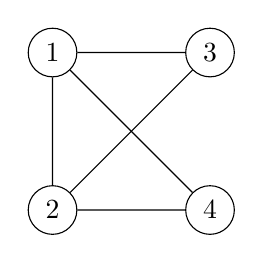
\begin{tikzpicture}[scale = 2]
		\node (1)[circle, draw] at (0,0){1};
		\node (2)[circle, draw] at (0,-1){2};
		\node (3)[circle, draw] at (1,0){3};
		\node (4)[circle, draw] at (1,-1){4};
		\draw (1)--(2)--(4)--(1);
		\draw (2)--(3)--(1);
	\end{tikzpicture}
\end{center}
\begin{figure}[H]
  \begin{center}
      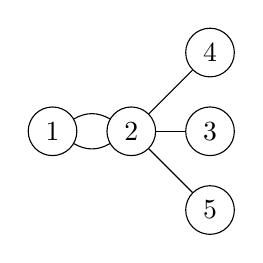
\begin{tikzpicture}
      \node (1)[circle, draw] at (0,0){1};
      \node (2)[circle, draw] at (1,0){2};
      \node (3)[circle, draw] at (2,0){3};
      \node (4)[circle, draw] at (2,1){4};
      \node (5)[circle, draw] at (2,-1){5};
      \draw [bend left](1)to(2);
      \draw [bend left](2)to(1);
      \draw (2)--(3);
      \draw (2)--(4);
      \draw (2)--(5);
    \end{tikzpicture} 
  \end{center}
	\caption{Questo non è un grafo}
\end{figure}
\subsection{Sottografi}
\definizione{Sottografo}{
	Siano $ G = \left(V, E\right) $ e $ G'=\left(V', E '\right) $ due grafi. Diciamo che $ G' $ è un sottografo di $ G $ se $ V' \in V $ e $ E' \subset E$
}
\definizione{Sottografo indotto}{
	Siano $ G = \left(V, E\right) $ un grafo. Diciamo che $ G' $ è un sottografo di $ G $ indotto da $ V' $
	\[
		G\left[V'\right]  = \left(V', E \cap \binom{V'}{2}\right)
	\]
}
\subsection{Morfismi di grafi}
\definizione{Morfismo di grafo}{
	Siano $ G \left(V, E\right) $ e $ G' = \left(V', E'\right) $. Una $ f: V \to  V' $ una \underline{funzione iniettiva} si dice \underline{morfismo} da $ G $ in $ G' $ se \underline{preserva i lati}
}

\definizione{Isomorfismo di grafo}{
	Siano $ G \left(V, E\right) $ e $ G' = \left(V', E'\right) $. Una $ f: V \to  V' $ una \underline{funzione iniettiva} si dice \underline{isomorfismo} da $ G $ in $ G' $ se:
	\begin{itemize}
		\item $ f $ è bigettiva
		\item $ f $ è un morfismo
		\item $ f^{-1}: V \left(G'\right) \to  V \left(G\right) $ è un morfismo
	\end{itemize}
	se esiste un isomorfismo da $ G $ e $ G' $ allora sono \underline{isomorfi}. Scriveremo che $ G \cong G'$
}
\teorema{Condizione isomorfismo}{
	Sia $  G = \left(V, E\right) $ e $ G' = \left(V', E'\right) $ e sia $ f: V \to  V' $. Allora $ f  $ è un isomorfismo da $ G $ in $ G' $ se e solo se:
	\begin{itemize}
		\item $ f $ è bigettiva
		\item $ f\left(E\right) = E' $
	\end{itemize}
}
\subsubsection*{Dimostrazione}
Chiaramente la prima proprietà coincide con la prima. La seconda proprietà afferma che $ f $ è un morfismo.

\begin{minipage}[c]{0.30\textwidth}
	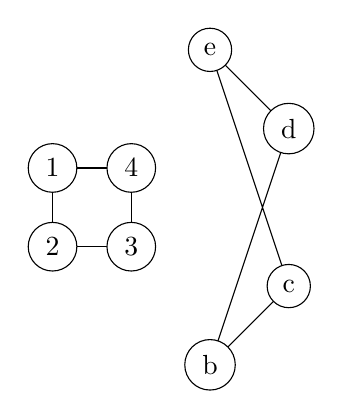
\begin{tikzpicture}
		\draw (0,0)node [draw,circle, fill = white] {1}--(0,-1) node [draw,circle, fill = white] {2} -- (1,-1) node [draw,circle, fill = white] {3} -- (1,0) node [draw,circle, fill = white] {4} -- cycle;
		\draw [shift={(2,-2.5)}](0,4)node [draw,circle, fill = white] {e}--(1,3)node [draw,circle, fill = white] {d}--(0,0)node [draw,circle, fill = white] {b}--(1,1)node [draw,circle, fill = white] {c}--cycle;
	\end{tikzpicture}

\end{minipage}
%
\begin{minipage}[c]{0.68\textwidth}
	\begin{minipage}[b]{0.48\textwidth}
		\centering
		\begin{align*}
			f:V & \to  V' \\
			1   & \to d   \\
			2   & \to b   \\
			3   & \to c   \\
			4   & \to e
		\end{align*}
		Quindi $ f $ è bigettiva
	\end{minipage}
	%
	\begin{minipage}[b]{0.48\textwidth}
		\centering
		\begin{align*}
			\left\{1,2\right\}  & \to \left\{ d,b\right\} \in  E' \\
			\left\{ 2,3\right\} & \to \left\{b,c\right\} \in  E'  \\
			\left\{3,4\right\}  & \to  \left\{c,e\right\} \in  E' \\
		\end{align*}
		Quindi preserva i lati
	\end{minipage}
\end{minipage}
\definizione{Passeggiate cammini e cicli}{
	Sia $  G \left(V, E\right) $ un grafo. Una successione finita ordinata $ \left(v_0,v_1,\ldots ,v_n\right) $ si verdici di $ G $ si dice:
	\begin{itemize}
		\item \underline{Passeggiata} se $ n = 0 $ oppure $  n \ge 1 $ e $ \left\{v_i, v_{i+1}\right\} \in E  \quad \forall i \in \left\{ 0,\ldots ,n-1\right\}$
		\item \underline{Cammino} se è una passeggiata in $ G $, ma non si ritorna mai sullo stesso vertice
		\item \underline{Ciclo} se è una passeggiata in $ G $ e:
		      \begin{itemize}
			      \item       $ n \ge 3 $
			      \item $ v_n = v_0 $
			      \item $ \left(v_0, \ldots , v_{n_1}\right) $ è un cammino
		      \end{itemize}
	\end{itemize}
}
\subsubsection*{Esempio}
\begin{center}
  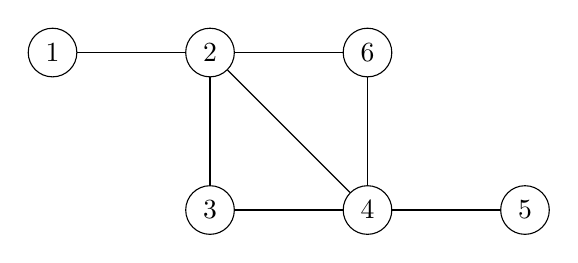
\begin{tikzpicture}
    \draw 
    (0,0)node(1)[ draw, circle, fill = white]{1}
    (2,0)node(2)[draw, circle, fill = white]{2}
    (4,0)node(6)[draw, circle, fill = white]{6}
    (4,-2)node(4)[draw, circle, fill = white]{4}
    (2,-2)node(3)[draw, circle, fill = white]{3}
    (6,-2)node(5)[draw, circle, fill = white]{5};
    %
    \draw (1)--(2);
    \draw (2)--(6);
    \draw (6)--(4);
    \draw (4)--(2);
    \draw (2)--(3);
    \draw (3)--(4);
    \draw (4)--(5);
\end{tikzpicture} 
\end{center}
\begin{minipage}[c]{0.48\textwidth}
  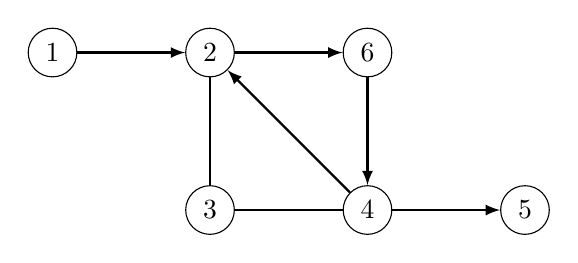
\begin{tikzpicture}
    \draw (0,0)node(1)[ draw, circle, fill = white]{1}
    (2,0)node(2)[draw, circle, fill = white]{2}
    (4,0)node(6)[draw, circle, fill = white]{6}
    (4,-2)node(4)[draw, circle, fill = white]{4}
    --(2,-2)node(3)[draw, circle, fill = white]{3}--(2,0)
    (4,-2)(6,-2)node(5)[draw, circle, fill = white]{5};
    \draw [-latex, thick](1)--(2);
    \draw [-latex, thick](2)--(6);
    \draw [-latex, thick](6)--(4);
    \draw [-latex, thick](4)--(2);
    \draw [-latex, thick](4)--(5);
\end{tikzpicture} 
\end{minipage}
%
\begin{minipage}[c]{0.48\textwidth}
  \begin{center}
      Cammino di lunghezza $ 5 $ 
    \[
      C \left(1,2,6,4,5\right)
    \] 
  \end{center}
\end{minipage}
\vskip3mm
\begin{minipage}[c]{0.48\textwidth}
  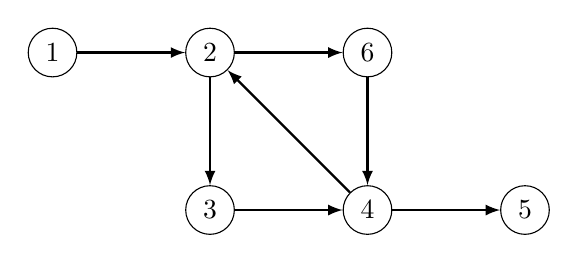
\begin{tikzpicture}
    \draw 
    (0,0)node(1)[ draw, circle, fill = white]{1}
    (2,0)node(2)[draw, circle, fill = white]{2}
    (4,0)node(6)[draw, circle, fill = white]{6}
    (4,-2)node(4)[draw, circle, fill = white]{4}
    (2,-2)node(3)[draw, circle, fill = white]{3}
    (6,-2)node(5)[draw, circle, fill = white]{5};
    %
    \draw [-latex, thick](1)--(2);
    \draw [-latex, thick](2)--(6);
    \draw [-latex, thick](6)--(4);
    \draw [-latex, thick](4)--(2);
    \draw [-latex, thick](2)--(3);
    \draw [-latex, thick](3)--(4);
    \draw [-latex, thick](4)--(5);
\end{tikzpicture} 
\end{minipage}
%
\begin{minipage}[c]{0.48\textwidth}
  \begin{center}
      Passeggiata di lunghezza $ 8 $ 
    \[
      P \left(1,2,6,4,2,3,4,5\right)
    \] 
  \end{center}
\end{minipage}
\vskip3mm
\begin{minipage}[c]{0.48\textwidth}
  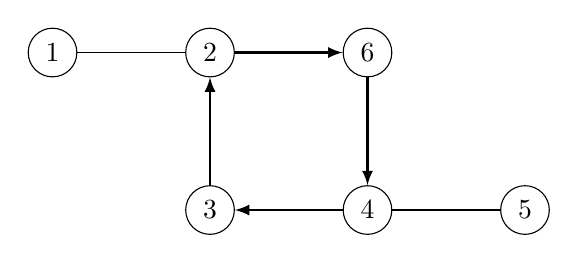
\begin{tikzpicture}
    \draw 
    (0,0)node(1)[ draw, circle, fill = white]{1}
    --(2,0)node(2)[draw, circle, fill = white]{2}
    (4,0)node(6)[draw, circle, fill = white]{6}
    (4,-2)node(4)[draw, circle, fill = white]{4}
    (2,-2)node(3)[draw, circle, fill = white]{3}
    (6,-2)node(5)[draw, circle, fill = white]{5};
    %
    \draw [-latex, thick](2)--(6);
    \draw [-latex, thick](6)--(4);
    \draw [-latex, thick](4)--(3);
    \draw [-latex, thick](3)--(2);
    \draw (4)--(5);
\end{tikzpicture} 
\end{minipage}
%
\begin{minipage}[c]{0.48\textwidth}
  \begin{center}
    Ciclo di lunghezza 4
    \[
      C \left(2,6,4,3\right)
    \] 
  \end{center}
\end{minipage}

\definizione{Confiungibilità}{
	Sia $ G = \left(V, E\right) $ un grafo e siano $ v,w \in V $. Diciamo che $ v $ è \underline{congiungibile} a $ w $ in $ G $ per cammini (o per passeggiate), se esiste una cammino (o una passeggiata) che parte da $ v $ e finisce in $ w $.
	\[
		\exists \left(v_0,\ldots ,v_n\right) \text{ t.c. } v_0 = v \text{ e } v_n = w
	\]
}
\teorema{Congiungibilità per cammino o passeggiata}{
	Se $ v $ e $ w $ sono congiungiungibili \underline{per passeggiate} in $ G $, allora lo  sono \underline{anche per cammini} e viceversa
}
\label{teocongiung} 
\subsubsection*{Dimostrazione}
\begin{itemize}
	\item Se $ v $ e $ k $ sono congiungibili per cammini, allora lo sono anche per passeggiate in quanto un cammino è una passeggiata
	\item Viceversa, se $ v $ e $ k $ sono congiungibili in passeggiata, posso scegliere la passeggiata più corta, evitando di ritornare sui miei passi
	      \begin{itemize}
		      \item Seleziono il seguente insime:
		            \[
			            \mathcal{P} := \left\{ Q | Q \text{ è una passeggiata in } G \text{ da } v \text{ a } w\right\}
		            \]
		            nota che $ P \not = \emptyset $  in quanto per hp esiste una passeggiata da $ v $ e $ w $
		      \item Definiamo anche il seguente insieme:
		            \[
			            \mathcal{A} := \left\{l\left(Q\right) \in  \N | Q \in  \mathcal{P}, l \left(Q\right) = n\text{ lati persorsi durante la passeggiata } Q\right\}
		            \]
		            Per lo stesso motivo di prima, anche $ \mathcal{A}\not = \emptyset  $
		      \item Grazie al teorema del buon ordinamento $ \exists p_0 = min\left(\mathcal{A}\right) $
		      \item Dimostriamo che $ p_0 $ è un cammino
		            \begin{itemize}
			            \item Supponiamo per assurdo che $ p_0 $ non sia un cammino.
			            \item Se $ p_0 $ non fosse un cammino allora potrei risparmiare lunghezza"tagliando la parte di cammino" che riporta allo stesso vertice
			            \item Tuttavia così facendo otterrei una passeggiata più corta di $ p_0 $, che per definizione è la passeggiata più corta di $ \mathcal{A} $, i che è un assurdo logico
		            \end{itemize}
	      \end{itemize}
\end{itemize}
\definizione{Grafi connessi}{
	Sia $ \sim  $ una relazione di equivalenza tale che
	\[
		v \sim  w \text{ se } v \text{ è connesso a } w
	\]
	detta $ \left[c\right]_{\sim } $ la classe dei vertici che soddisfano la relazione $ \sim $ a partire da $ c $, allora il sottografo indotto dai vertici di una tale classe è detto \underline{grafo delle componenti connesse}. Se un grafo ha una sola classe è detto \underline{grafo connesso}. In caso contrario è detto \underline{grafto sconnesso}
}
\subsubsection*{Esempio}
\vskip3mm
\begin{center}
	\begin{figure}[H]
		\begin{center}
			\begin{subfigure}{0.3\textwidth}
				\begin{center}
					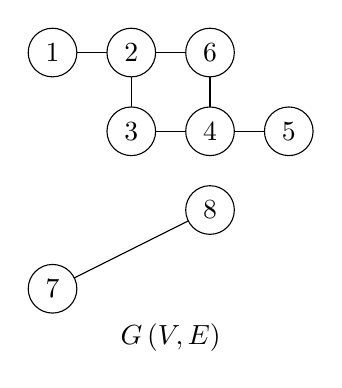
\begin{tikzpicture}
						\draw (0,0)node[ draw, circle, fill = white]{1}
						--(1,0)node[draw, circle, fill = white]{2}
						--(2,0)node[draw, circle, fill = white]{6}
						--(2,-1)node[draw, circle, fill = white]{4}
						--(1,-1)node[draw, circle, fill = white]{3}
						--(1,0)
						(2,-1)--(3,-1)node[draw, circle, fill = white]{5};
						\draw (0, -3)node[draw, circle, fill = white]{7}
						--(2, -2)node[draw, circle, fill = white]{8};
						\node at (current bounding box.south) [anchor = north] {$ G\left(V, E\right) $};
					\end{tikzpicture}
				\end{center}
			\end{subfigure}
			%
			\begin{subfigure}{0.3\textwidth}
				\begin{center}
					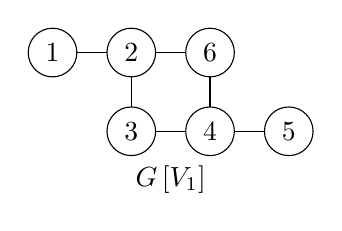
\begin{tikzpicture}
						\draw (0,0)node[ draw, circle, fill = white]{1}
						--(1,0)node[draw, circle, fill = white]{2}
						--(2,0)node[draw, circle, fill = white]{6}
						--(2,-1)node[draw, circle, fill = white]{4}
						--(1,-1)node[draw, circle, fill = white]{3}
						--(1,0)
						(2,-1)--(3,-1)node[draw, circle, fill = white]{5};
						--(2, -2)node[draw, circle, fill = white]{8};
						\node at (current bounding box.south) [anchor = north] {$ G\left[V_1\right] $};
					\end{tikzpicture}
				\end{center}
			\end{subfigure}
			%
			\begin{subfigure}{0.3\textwidth}
				\begin{center}
					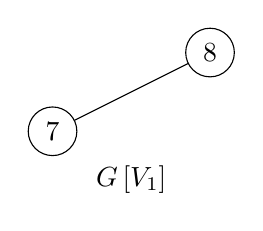
\begin{tikzpicture}
						\draw (0, -3)node[draw, circle, fill = white]{7}
						--(2, -2)node[draw, circle, fill = white]{8};
						\node at (current bounding box.south) [anchor = north] {$ G\left[V_1\right] $};
					\end{tikzpicture}
				\end{center}
			\end{subfigure}
		\end{center}
		\caption{A sinistra $ G $, a destra i sottografi connessi di $ G $}
	\end{figure}
\end{center}
\begin{align*}
	\left[1\right]_{\sim } & = \left\{ 1,2,3,4,5,6\right\} = V_1 \\
	\left[7\right]_{\sim } & = \left\{7,8\right\} = V_2
\end{align*}
\subsection{Grafi 2-connessi e hamiltoniani}
Definiamo innanzitutto delle operazioni sui grafi:
\definizione{Operazioni sui grafi}{
	Sia $G=(V, E)$ un grafo, definiamo alcuni grafi costruiti a partire da $G$ :
	\begin{itemize}
		\item  \textit{Cancellazione di un lato} se $e \in E$ denotiamo
		      \[
			      G - e=(V, E \backslash\{e\})
		      \]
		\item  \textit{Aggiunta di un lato} se $e \in\left(\begin{array}{l}V \\ 2\end{array}\right) \backslash E$ denotiamo
		      \[
			      G+e=(V, E \backslash\{e\})
		      \]
		\item  \textit{Cancellazione di un vertice} se $v \in V$ denotiamo
		      \[
			      G - v=(V \backslash\{v\},\{e \in E \mid v \notin e\})
		      \]
		\item  \textit{Divisione di un lato} se $e=\{u, v\} \in E$ denotiamo
		      \[
			      G \% e=(V \cup\{z\}, E \backslash\{e\} \cup\{\{u, z\},\{v, z\}\})
		      \]
		      essendo $z \notin V$.
	\end{itemize}
}
\definizione{Grafo 2-connesso}{
	Una grafo $ F $ si dice \underline{2-connesso} se ha almeno tre vertici e
	\[
		\forall  v \in  V \left(G\right)\quad G-v\text{ è connesso }
	\]
	ossia qualsiasi vertice io tolga ottengo un grafo connesso
}
\definizione{Grafo hamiltoniano}{
	Sia $ G $ un grafo. Un ciclio in $ G $ che attraversa tutti i vertici di $ G $ è detto \underline{ciclo hamiltoniano} in $ G $. Se $ G $ ammette almeno un ciclo hamiltoniano, allora $ G $ è detto \underline{grafo hamiltoniano}
}
Nota che un grafo hamiltoniano è sempre anche 2-connesso
\subsection{Gradi di un vertice e teoremi correlati}
\definizione{Grafo finito}{
	Un grafo si dice finito se il suo \underline{numero di vertici} è finito
}
Nota che un grafo finito ha anche un numero di lati finito. Tuttavia un grafo con numero finito di lati può essere anche infinito
\definizione{Grado di un vertice}{
	Sia $ G = \left(V, f\right) $ un grafo finito e sia $ v \in  V $. Definiamo il \underline{grado} $ deg_G\left(V\right) $ di $ v  $in $ G $ ponendo:
	\[
		deg_G\left(v\right) = \left|\left\{e \in  E\right\}| v \in  e\right|
	\]
	intuitivamente indica il \underline{numero di lati che escono} da $ v $
}
\teorema{Somma dei gradi}{
	Sia $ G = \left(V, f\right) $ un grafo finito. Allora vale che
	\[
		\sum_{v \in  V}\operatorname{deg}_G \left(v\right)  = 2 \left|E\right|
	\]
}
\label{teosommadeigradi} 
Intuitivamente, ogni volta che aggiungo un lato, ogni lo score dei due vertici che collega si alzerà di 1 per ogni vertice.
\subsubsection*{Dimostrazione}
Definisco innanzitutto la matrice di adiacenza nel seguente modo:
\[
	m_{ij} =
	\begin{cases}
		1 & \text{ se } v_i \in  e_j      \\
		0 & \text{ se } v_i \not \in  e_j
	\end{cases}
\]
immaginati di avere sulla ascisse il vertice e sulle ordinate il lato. Se in posizione $ \left(i,j\right) $ c'è un 1, vuol dire che il $ j $-esimo lato è collegato all'$ i $-esimo vertice
\begin{itemize}
	\item Immagina di sommare tutti gli uni presenti in matrice.
	\item Puoi procedere sommando prima colonne e poi righe o viceversa. La somma è chiaramente uguale
	      \[
		      \sum_{i=1}^{n} \left(\sum_{j=1}^{k} m_{ij}\right) = \sum_{j=1}^{k} \left(\sum_{i=1}^{n} m_{ij}\right)
	      \]
	      assumendo che vi siano $ n $ vertici e $ k $ lati
	\item La quantità a sinistra è pari alla somma dei gradi (fisso un vertice e conto quali lati lo contengono)
	\item La quantità della sommatoria interna a destra è sempre pari a 2 (fisso un lato e contro quanti vertici lo contengono, sempre 2). Visto che la sommatoria esterna varia da $ 1 $ a $ k $, dove $ k $ è il numero dei lati, allora la quantità di destra è pari a $ 2 \left|E\right| $
	      \[
		      \sum_{i=1}^{n} \operatorname{deg} \left(v_i\right) = 2 \left|E\right|
	      \]
\end{itemize}
\teorema{Teorema delle strette di mano}{
  Il numero di vertici \underline{di grado dispari} in un grafo \underline{finito} è \underline{pari}
}
\label{teostrettedimano}
\subsubsection*{Dimostrazione}
Consideriamo i due insiemi contenenti i vertici pari e dispari: 
\begin{align*}
  P:= \left\{v \in V | \operatorname{deg}_G\left(v\right) \text{ è pari }\right\} && D:= \left\{v \in V | \operatorname{deg}_G\left(v\right) \text{ è dispari }\right\}
\end{align*}
ora so che la somma di questi gradi sarà uguale alla somma di tutti i gradi: 
\[
  \sum_{v \in  P} \operatorname{deg}_G\left(v\right) + \sum_{v \in  D} \operatorname{deg}_G\left(v\right) = \sum_{v \in  V} \operatorname{deg}_G\left(v\right) = \underbracket[0.1ex]{2 \left|E\right|}_{\text{ teo \ref{teosommadeigradi}}}
\]
A questo punto , girando l'uguaglianza ottengo che : 
\[
   \sum_{v \in  D} \underbracket[0.1ex]{\operatorname{deg}_G\left(v\right)}_{\text{ dispari }} = \overbracket[0.1ex]{\sum_{v \in  P} \operatorname{deg}_G\left(v\right)}^{\text{ pari }} + \overbracket[0.1ex]{2 \left|E\right|}^{\text{ pari }}
\]
\begin{itemize}
  \item Il membro di destra è pari (somma di numeri pari è pari)
  \item La somma di numeri dispari è pari se e solo se \underline{il numero di numeri dispari} è \underline{pari}
\end{itemize}
\definizione{Foglia}{
	Sia $ G = \left(V, E\right) $ un grafo . Un vertice $ v \in  V $ si dice \underline{foglia} di $ G $ se
	\[
		deg\left(v\right) = 1
	\]
}
\teorema{Foglie in grafo 2 connesso}{
	Sia $ G = \left(V, E\right) $ un grafo \underline{2-connesso}. Allora $ G $ \underline{non ha foglie}
}\label{foglie 2-connesso}
\subsubsection*{Dimostrazione}
Supponiamo per assurdo che esista una foglia di $ G $, ossia $ \exists v \in V \text{ t.c. } deg\left(v\right) = 1 $. Se considero il grafo $ G - w $ dove $ w \in \left\{w,v\right\} $, allora chiaramente ottengo un grafo sconnesso
\teorema{Foglie grafo hamiltoniano}{
	Se $ G = \left(V, E\right) $ è un grafo hamiltoniano allora \underline{non ha foglie}
}
\subsubsection*{Dimostrazione}
Il fatto che un grafo sia hamiltoniano implica che sia $ 2-connesso $, allora per teo \ref{foglie 2-connesso} ho che il grafo \underline{non ha foglie}
\vskip3mm
Nota che non è vero che se un grafo è connesso e senza foglie allora è 2-connesso o hamiltoniano
\subsubsection*{Categorie di grafi}
\begin{center}
	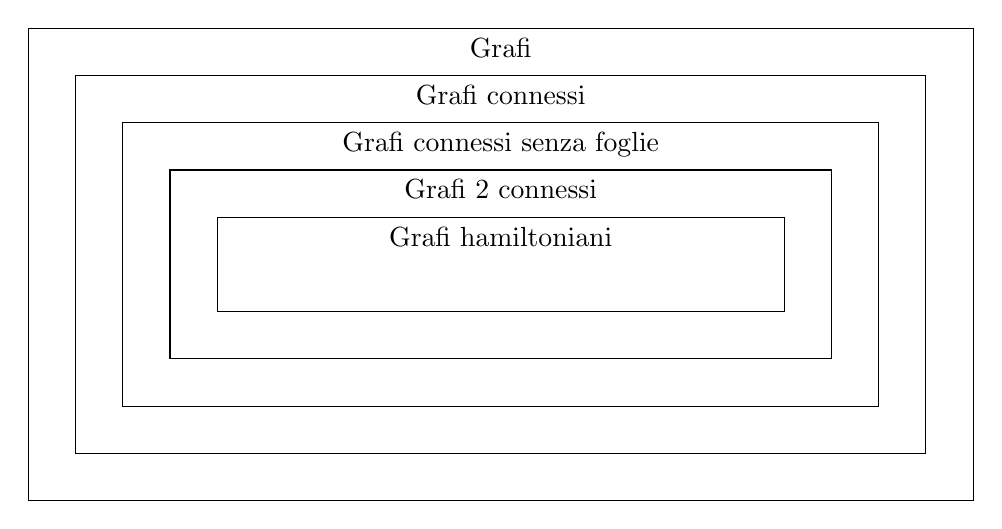
\begin{tikzpicture}[scale = 1.2]
		\draw (0,0)rectangle(10,5);
		\draw (0.5,0.5)rectangle(9.5,4.5);
		\draw (1,1)rectangle(9,4);
		\draw (1.5,1.5)rectangle(8.5,3.5);
		\draw (2,2)rectangle(8,3);
		\node [anchor = north ] at (5,5) {Grafi};
		\node [anchor = north ] at (5,4.5) {Grafi connessi};
		\node [anchor = north ] at (5,4) {Grafi connessi senza foglie};
		\node [anchor = north ] at (5,3.5) {Grafi 2 connessi };
		\node [anchor = north ] at (5,3) {Grafi hamiltoniani};
	\end{tikzpicture}
\end{center}
\teorema{Proprietà grafi isomorfi}{
	Siano $ G  $ e $ G' $ grafi finiti. Supponiamo $ G \cong G' $. Allora valgono:
	\begin{itemize}
		\item $ \text{ Score}\left(G\right) = \text{ Score} \left(G'\right) $
		\item $ G $ e $ G' $ hanno lo stesso numero di \underline{componenti connesse}
		\item $ G $ è 2-connesso $ \Leftrightarrow G' $ è 2 connesso
		\item $ G $ è hamiltoniano $ \Leftrightarrow G' $ è hamiltoniano
		\item $ G $ e $ G' $ hanno lo stesso numero di sottografi che sono 3-cicli, 4-cicli,$ \ldots  $
	\end{itemize}
}
\subsection{Verificare se uno score esiste o meno}
\subsubsection*{Osservazione}
Se conosco lo score di un grafo allora conosco anche il numero di vertici e lati:
\begin{itemize}
	\item Il numero di vertici è il numero di entrate nello score
	\item La somma delle entrare dello score è il numero di lati presenti
\end{itemize}
\teorema{Condizione esistenza score 1}{
	Sia $ d = \left(d_1,d_1,\ldots ,d_n\right) \in  \N ^{n} $ con $ n \ge  1 $ con $ d_1 \le  d_2 \le  \ldots \le  d_n $ lo score di un grafo. Se
	\[
		d_n > n -1
	\]
	\underline{non può essere lo score} di alcun grafo
}
\begin{itemize}
	\item Se la $ n $-upla è lunga $ n $, allora vuol dire che il grafo ha $ n $ vertici
	\item Ogni vertice può essere collegato con al massimo $ n-1 $ vertici
\end{itemize}
Nota che se ho uno score con 0:
\[
	d = \left(0,0,0,1,1,2,2,2,3,4,9\right)
\]
in questo caso lo score è lungo $ n = 11 $ dunque non posso provare l'inesistenza dello score dato che $ 9 \not \ge 11 $. Tuttavia posso considerare lo score senza gli 0, in quanto ogni vertice con grado 0 non è collegato a nulla. Dato che lo score
\[
	d = \left(1,1,2,2,2,3,4,9\right)
\]
non esiste, allora non esiste nemmeno lo score iniziale
\teorema{Condizione esistenza score 2}{
	Siano $ h, k \in  \N \setminus \left\{0\right\} $, sia $ n :=h + k $ e sia $ d \in  \N ^{n} $ tale che :
	\[
		d = \left(\underbracket[0.1ex]{d_1, d_2, \ldots ,d_h}_{h \text{ volte }}, \underbracket[0.1ex]{n-1, n-1, \ldots , n-1}_{k \text{ volte }}\right)
	\]
	allora se $ d_1 < k $, allora $ \not \exists G $ con score $ d $
}
\subsubsection*{Dimostrazione}
Supponiamo per assurdo che eiste $ G \left(V, E\right) $ con score $ d $. Se ho $ k $ vertici collegati a $ n-1 $ vertici, ossia a tutti, non posso avere nemmeno un vertice che \underline{non} sia collegato ad \underline{almeno $ k $} vertici
\subsubsection*{Esempio}
Considera la stringa:
\[
	d = \left(0,0,0,2,3,3,3,3,3,3,4,10,10,10\right)
\]
quindi $ n = 14 $
\begin{itemize}
	\item Metodo 1: non posso dire nulla in quanto $ d_1 = 10 \not \ge n-1 = 14 $
	\item Tutta via posso trimmare via gli zero davanti e appricare il metodo 3
	      \[
		      d' = \left(2,3,3,3,3,3,3,4,10,10,10\right)
	      \]
\end{itemize}
\teorema{Condizione esitenza score 3}{
	Sia $  n \in  \N  $  e $ n \ge  3 $, sia $ d = \left(d_1,\ldots ,d_n\right) \in  \N ^{n} $ tale che
	\[
		d_1 \le  d_2 \le  \ldots \le  d_n
	\]
	e sia $ L \in  \N  $ definita ponendo
	\[
		L = \left|\left\{ i \in  \left\{1,2,\ldots , n-2\right\}|d_i \ge 2\right\}\right|
	\]
	ossia calcolo quante entrate nello score sono maggiori o uguali a 2, eccetto le ultime 2. Allora se
	\[
		L < d_{n-1} + d_n - n
	\]
	allora \underline{non esiste} un grafo con tale score
}
L'idea intuitiva è la seguente:
\begin{itemize}
	\item Immaginati di porre gli utlimi due vertici dello score $ d_{n-1}, d_n $
	\item A questo punto i lati che escono da questi devono confluire in alcuni vertici, ma se questi sono troppo pochi allora ci devono essere alcuni vertici collegati da entrambi $ d_{n-1} $ e $ d_{n} $
\end{itemize}
\begin{center}
	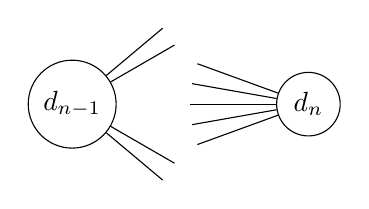
\begin{tikzpicture}
		\node (1)[draw, circle] at (0,0) {$ d_{n-1} $};
		\node (2)[draw, circle] at (3,0) {$ d_{n} $};
		\draw (1)--(30:1.5);
		\draw (1)--(40:1.5);
		\draw (1)--(-40:1.5);
		\draw (1)--(-30:1.5);
		\draw (2)--++(200:1.5);
		\draw (2)--++(180:1.5);
		\draw (2)--++(190:1.5);
		\draw (2)--++(160:1.5);
		\draw (2)--++(170:1.5);
	\end{tikzpicture}
\end{center}
\teorema{Condizione esitenza score 4}{
	Se il vettore $  d \in  \N  ^{n} $ possiede un numero dispari di componenti dispari allora \underline{non} può essere lo score di un grafo, grazie al \underline{lemma delle strette di mano}
}
\teorema{Prerequisito teorema dello score}{
	Sia $ n \in  \N  \setminus \left\{ 0\right\} $ e sia $  d = \left(d_1, \ldots , d_n\right)\in  \N^{n} $ tale che $ d_1 \le  d_2 \le  \ldots \le  d_n  \le  2$. Valgono le seguenti:
	\begin{itemize}
		\item Se $ d = \left(0,0,\ldots ,0,2\right) $ oppure $ d = \left(0,0,\ldots , 2,2\right) $ allora \underline{non esiste}
		\item Se $ d = \left(0,\ldots ,0\right) $ p $ d = (\underbracket[0.1ex]{0,\ldots, 0}_{n-m \text{ volte }} ,\underbracket[0.1ex]{2,\ldots ,2}_{m \text{  volte }}) $ allora \underline{esiste}. In quest'ultimo caso basta prendere un $ m $ ciclo e $ n-m $ vertici non collegati a nulla
		\item Se compare almeno una volta $ 1 $, allora se compare un numero di volte dispari il grafo non esiste (\textit{teo delle strette di mano}). Supponiamo di avere un numero pari di uni:
		      \[
			      d = (\underbracket[0.1ex]{0,\ldots ,0}_{h \text{ volte }},\underbracket[0.1ex]{1,1}_{2 \text{ volte }},\underbracket[0.1ex]{1,\ldots ,1}_{2k \text{ volte }},\underbracket[0.1ex]{2,\ldots ,2}_{m \ge  0})
		      \]
	\end{itemize}
	\begin{center}
		\textbox{
			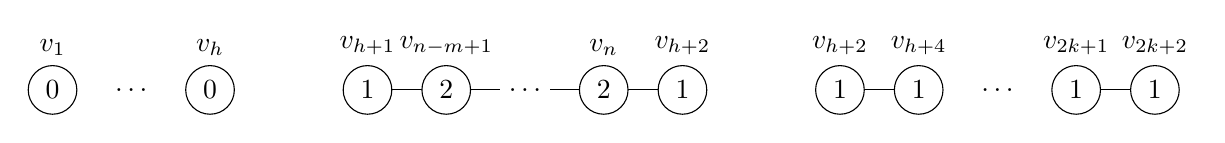
\begin{tikzpicture}
				\node [draw, circle, label = $ v_1 $]at(0,0) {0};
				\node at(1,0) {$ \ldots  $};
				\node [draw, circle, label = $ v_h $]at(2,0) {0};
				\draw (4,0) node [draw, circle, fill = white, label = $ v_{h+1}$] {1}
				-- (5,0)node [draw, circle, fill = white, label = $ v_{n-m+1}$] {2}
        -- (6,0)node [fill = white] {$ \ldots  $}
				-- (7,0) node [draw, circle, fill = white, label = $ v_{n}$] {2}
				-- (8,0)node [draw, circle, fill = white, label = $ v_{h+2}$] {1};
				%
        \draw (10,0)	node [draw, circle, fill = white, label = $ v_{h+2}$] {1}
        --(11,0)	node [draw, circle, fill = white, label = $ v_{h+4}$] {1}
        (12,0) [fill = white]node {$ \ldots  $}
        (13,0)	node [draw, circle, fill = white, label = $ v_{2k+1}$] {1}
        --(14,0)	node [draw, circle, fill = white, label = $ v_{2k+2}$] {1};
			\end{tikzpicture}}
		\textit{Grafo "canonico"} dell'ultimo punto
	\end{center}
}\label{score banale} 
\teorema{Teorema dello score}{
  Sia $  n \in  \N  $ con $ n \ge 2 $ e sia $ d = \left(d_1, \ldots , d_n\right) \in  \N ^{n} $ tale che $ d_1 \le  \ldots \le d_n \le  n-1 $. Definiamo il vetore $ d' =\left(d_1',\ldots , d'_{n-1} \in  \N ^{n-1}\right) $, togliendo l'ultimo elemento di $ d $ in modo tale che: 
  \[
  d_i' = 
  \begin{cases}
    d_i & \text{ se } i < n-d_n\\
    d_i - 1 & \text{ se } i \ge  n-d_n
  \end{cases}
  \]
  per $ i \in  \left\{1,\ldots ,n-1\right\} $. Allora 
  \begin{center}
    $ d $ esiste $ \Leftrightarrow  $ esiste $ d' $
  \end{center}
}
Nota che il teorema può essere applicatore iterativamente su anche su $ d' $ finche non otteniamo uno score banale. 
\subsubsection*{Esempio}
Consideriamo lo score 
\[
  \left(2,2,2,2,3,3,3,5,6\right)
\]
\begin{center}
  \begin{tabular}{|l l|}
    \hline
    Score & Dati \\
    \hline
    $ (2,2,\underbracket[0.1ex]{2,2,3,3,3,5}_{\text{ range }},6) $ & $ n = 9, n - d_m = 3 $ \\ 
    \hline
    $ (2,2,1,1,2,2,2,4) $ & \multirow{2}{*}{$ n=8, n-d_m = 4 $} \\ 
    $ (1,1,2,\underbracket[0.1ex]{2,2,2,2}_{\text{ range }},4) $ &  \\ 
    \hline
    $ (1,1,2,1,1,1,1) $ & \multirow{2}{*}{Ottengo score banale} \\ 
    $ \left(1,1,1,1,1,1,2\right) $ &  \\ 
    \hline
  \end{tabular}
\end{center}
Come visto in teo \ref{score banale} esiste un grafo con score $ \left(1,1,1,1,1,1,2\right) $, allora posso affermare che ne esiste uno con score $ \left(2,2,2,2,3,3,3,5,6\right) $. Posso ora costruire un grafo con quest'ultimo score procedendo così:
\begin{itemize}
  \item Nella tabella ho ottenuto i seguenti score secondo l'algoritmo dello Score: 
    \begin{align*}
      d &= \left(2,2,2,2,3,3,3,5,6\right) \\
      d' &= \left(1,1,2,2,2,2,2,4\right) \\ 
      d'' &= \left(1,1,1,1,1,1,2\right)
    \end{align*}
  \item Disegno grafo canonico dell'ultimo score:
    \begin{center}
          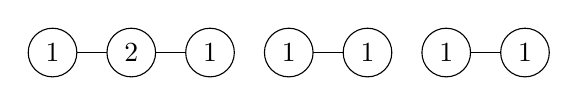
\begin{tikzpicture}[every node/.style={draw,circle, fill = white}]
          \draw  (0,0)[circle] node {1}
          --++(1,0)node{2}
          --++(1,0)node{1}
          ++(1,0)node{1}
          --++(1,0)node{1}
          ++(1,0)node{1}
          --++(1,0)node{1};
        \end{tikzpicture} 
    \end{center}
  \item Aggiungo il vertice che ho tolto nell'ultimo passaggio. Lo collego in maniera tale da riscostruire le differenze con l'ultimo score
    \begin{center}
          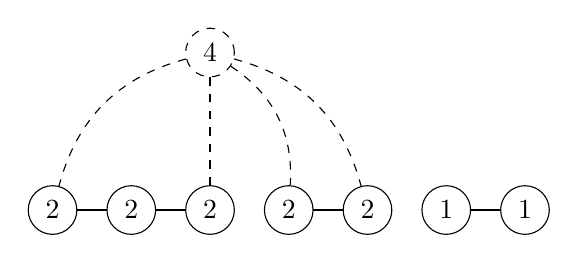
\begin{tikzpicture}[every node/.style={draw,circle, fill = white}]
            \draw  (0,0) node(a) {2}
            --++(1,0)node(b){2}
            --++(1,0)node(c){2}
              ++(1,0)node(d){2}
            --++(1,0)node(e){2}
              ++(1,0)node(f){1}
            --++(1,0)node(g){1};
            \node [dashed](h) at (2,2) {4};
            \draw [dashed ,bend right](h)to(a);
            \draw [dashed](h)to(c);
            \draw [dashed ,bend left](h)to(d);
            \draw [dashed ,bend left](h)to(e);
        \end{tikzpicture} 
    \end{center}
  \item Ripeto iterativamente: 
        \begin{center}
          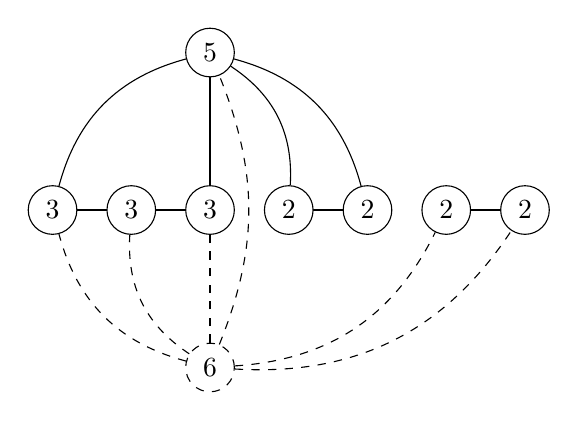
\begin{tikzpicture}[every node/.style={draw,circle, fill = white}]
            \draw  (0,0) node(a) {3}
            --++(1,0)node(b){3}
            --++(1,0)node(c){3}
              ++(1,0)node(d){2}
            --++(1,0)node(e){2}
              ++(1,0)node(f){2}
            --++(1,0)node(g){2};
            \node (h) at (2,2) {5};
            \draw [bend right](h)to(a);
            \draw (h)to(c);
            \draw [bend left](h)to(d);
            \draw [bend left](h)to(e);
            %
            \node [dashed](i) at (2,-2) {6};
            \draw[dashed, bend left](i)to(a);
            \draw[dashed, bend left](i)to(b);
            \draw[dashed](i)to(c);
            \draw[dashed,bend angle = 22, bend right](i)to(h);
            \draw[dashed, bend right](i)to(f);
            \draw[dashed, bend right](i)to(g);
        \end{tikzpicture} 
    \end{center}
\item Il grafo ottenuto tramite la ricostruzione arritrovo e quindi il seguente: 
        \begin{center}
          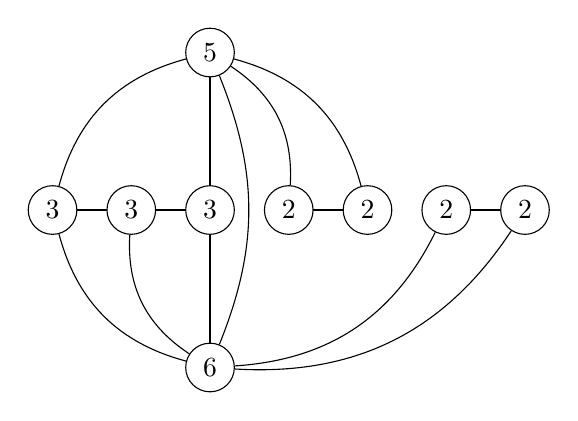
\begin{tikzpicture}[every node/.style={draw,circle, fill = white}]
            \draw  (0,0) node(a) {3}
            --++(1,0)node(b){3}
            --++(1,0)node(c){3}
              ++(1,0)node(d){2}
            --++(1,0)node(e){2}
              ++(1,0)node(f){2}
            --++(1,0)node(g){2};
            \node (h) at (2,2) {5};
            \draw [bend right](h)to(a);
            \draw (h)to(c);
            \draw [bend left](h)to(d);
            \draw [bend left](h)to(e);
            %
            \node (i) at (2,-2) {6};
            \draw [bend left](i)to(a);
            \draw [bend left](i)to(b);
            \draw (i)to(c);
            \draw [bend angle = 22, bend right](i)to(h);
            \draw [bend right](i)to(f);
            \draw [bend right](i)to(g);
        \end{tikzpicture} 
    \end{center}

\end{itemize}
\section{Esercizi}
\subsection{Esercizio induzione}
Dimostrare per induzione su $ n \ge  0 $ che vale la proprietà:
\[
	\sum_{k=0}^{n} k! k = \left(n+1\right)! -1 \quad \forall  n > 0
\]
\begin{itemize}
	\item \textit{Caso base}
	      \[
		      \sum_{k=0}^{0} k! k = 1 - 1 \rightarrow \text{ \checkmark }
	      \]
	\item \textit{Passo induttivo} suppongo la proprietà vera per $ n-1 $:
	      \[
		      n! n +\sum_{k=0}^{n-1} k!k = n! n +\left[\left(n-1 + 1\right)! -1\right]  = n!n+\left[n! -1\right] = n! \left(n + 1\right) - 1 = \left(n +1\right)! -1
	      \]
\end{itemize}
\subsection{Alberi e foreste}
\definizione{Alberi e foreste}{
	Un grafo si dice \underline{albero} se è un grafo \underline{connesso senza cicli}. Una \underline{foresta} è un grafo \underline{senza cicli}
}
Nota che un grafo è una foresta solo se le sue componenti connesse sono tutte alberi
\teorema{Caratterizzazione alberi}{
	Sia $ T =\left(V, E\right) $ un grafo (non necessariamente finito). Le seguenti affermazioni sono equivalenti:
	\begin{itemize}
		\item $ T $ è un albero
		\item Per ogni $ v , v' \in  V $, esiste un unico cammino in $ T $ che congiunge $ v $ a $ v' $
		\item $ T $ è connesso ma $ \forall  e \in  E $ il grafo $ T - e $ è sconnesso
		\item $ T $ non ha cicli e  $ \forall  e \in  \binom{V}{2} \setminus  E $ il grafo $ T + e $ ha almeno un ciclo
	\end{itemize}
}
\teorema{Foglie e alberi}{
	Sia $ T $ un albero finito avente almeno due vertici. Allora $ T $ possiede \underline{almeno due foglie}
}
Nota che il teorema è falso per i grafi \underline{non finiti}:
\vskip3mm
\begin{center}
	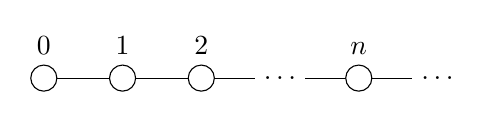
\begin{tikzpicture}
		\draw (0,0) node [draw, circle, fill = white, label = $ 0 $] {}
		-- (1,0) node [draw, circle, fill = white, label = $ 1 $] {}
		-- (2,0) node [draw, circle, fill = white, label = $ 2 $] {}
		-- (3,0) node [fill = white]{$ \ldots  $}
		-- (4,0) node [draw, circle, fill = white, label = $ n $] {}
		-- (5,0) node [fill = white]{$ \ldots  $};
	\end{tikzpicture}
\end{center}
\vskip3mm
oppure
\vskip3mm
\begin{center}
	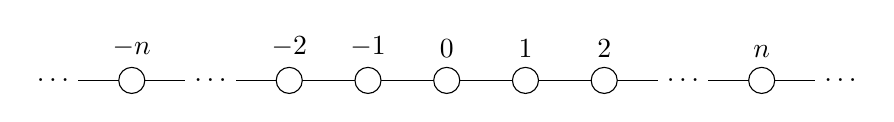
\begin{tikzpicture}
		\draw
		(-5,0) node [fill = white] {$ \ldots  $}
		--(-4,0) node [draw, circle, fill = white, label = $ -n $] {}
		--(-3,0) node [fill = white] {$ \ldots  $}
		--(-2,0) node [draw, circle, fill = white, label = $ -2 $] {}
		--(-1,0) node [draw, circle, fill = white, label = $ -1 $] {}
		--(0,0) node [draw, circle, fill = white, label = $ 0 $] {}
		-- (1,0) node [draw, circle, fill = white, label = $ 1 $] {}
		-- (2,0) node [draw, circle, fill = white, label = $ 2 $] {}
		-- (3,0) node [fill = white]{$ \ldots  $}
		-- (4,0) node [draw, circle, fill = white, label = $ n $] {}
		-- (5,0) node [fill = white]{$ \ldots  $};
	\end{tikzpicture}
\end{center}
\hypertarget{teoeulerografi}{}
\teorema{Formula di eulero per gli alberi}{
  Sia $ T \left(V, E\right) $ un grafo \underline{finito e connesso}. Allora 
  \[
  T \text{ è un albero } \Leftrightarrow \left| V\right| = \left|E\right| + 1
  \]
}
\subsubsection*{Dimostrazione $ \Rightarrow  $} 
Procediamo per induzione su $ \left|V\right| \ge  1 $
\begin{itemize}
  \item \textit{Base induzione} $ V = 1 $, non può avere lati dunque vale l'hp \checkmark
  \item \textit{Ipotesi induttiva} un albero con $ n $ vertici soddisfa la hp, ossia vale che $ \left|V\right| = \left|E\right| + 1 $ 
    \begin{itemize}
      \item So che ogni albero con $ \left|V\right| \ge 2 $ ha almeno due foglie
      \item So che se tolgo una foglia ad un albero questo rimane un albero
      \item Dunque tolgo una foglia all'albero $ T $, ricadendo nell'ipotesi induttiva 
        \[
          \left|V \left(T-v\right)\right| - 1 = \left|E \left(T-v\right)\right|
        \]
      \item Tuttavia, rimuovendo una foglia tolgo a $ T $ un vertice e un lato, dunque vale che 
        \[
          \left|V\left(T-v\right)\right| = \left|V \left(T\right)\right| -1 \quad \quad \left|E \left(T-v\right)\right| = \left|E \left(T\right)\right|-1
        \]
      \item Sostituendo nella prima equazione, ottengo che 
        \[
          \left|V \left(T\right)\right| -1 = \left|E \left(T\right)\right|
        \]
    \end{itemize}
\end{itemize}
\subsubsection*{Dimostrazione $ \Leftarrow  $}
Procediamo per induzione su $ \left|V\right| \ge 1 $
\begin{itemize}
  \item \textit{Base induzione} $ V =1 $ chiaramente verificata come prima \checkmark
  \item \textit{Ipotesi induttiva} un grafo finito per cui vale $ \left|V\right| = \left|E\right| + 1 $ è un \underline{albero}
    \begin{itemize}
      \item Devo dimostrare che il grafo ha almeno una foglia: supponiamo per assurdo che non la abbia 
        \[
          2 \left|V\right| - 2 =\underbracket[0.1ex]{2 \left(\left|V\right| - 1\right) }_{\text{per hp}} =\overbracket[0.1ex]{ 2 \cdot \left|E\right| = \sum \deg \left(v\right)}^{\text{ teo \hyperlink{teosommadeigradi}{somma gradi} }} \underbracket[0.1ex]{\ge 2 \left|V\right|}_{\text{ no foglie }}
        \]
      \item Tuttavia si noti come si è ottenuto un assurdo logico in quanto se confrontiamo il membro di estrema sinistra con quello di estrema destra otteniamo che 
        \[
                2 \left|V\right| -2 \ge  2 \left|V\right| 
        \]
        l'assunzione \underline{falsa} è che \underline{non esistano foglie}
        \item Dunque considero il grafo $ T - v $ dove $ v $ è la foglia di cui abbiamo dimostrato l'esistenza
        \item Mi basta dimostrare che aggiungendo $ v $ a $ T -v $ non introduco cicli: 
          \begin{itemize}
            \item $ v $ è una foglia, quindi un ciclo non può passare per una foglia
            \item Dato che per hp induttiva $ T-v $ è un albero, non ha cicli
            \item Per questa ragione anche $ T $ non ha cicli, quindi $ T $ è connesso e senza cicli, ossia \underline{un albero}
          \end{itemize}
    \end{itemize}
\end{itemize}
Quest'ultimo teorema ha un importante corollario: 
\teorema{Corollario 1 a teorema di Eulero per i grafi}{
  Sia $ n \in  \N \setminus \left\{0\right\} $ e sia $ d = \left(d_1, \ldots ,d_n\right) \in n \N ^{n} $. Allora esiste un albero con score $ d $ se e soltanto se è soddisfatta la relazione di eulero: 
  \[
  \left|V\right| -1 = \left|E\right| = \frac{1}{2} \sum_{i=1}^{\left|V\right|} d_i
  \]
}
\subsubsection*{Forzatura alla disconnessione}
\teorema{Corollario 2 a teorema di Eulero per i grafi}{
  Sia $ n \in \N  \setminus \left\{0\right\} $ e sia $ d \left(d_1, \ldots , d_n\right) \in  \N ^{n} $ . Se vale 
  \[
  \left|E\right| = \frac{1}{2} \sum_{i=1}^{n} d_i < n-1
  \]
  allora tutti i grafi che hanno score uguele a $ d $ sono \underline{sconnessi}
}
Informalmente, pensa che per un albero vale la relazione di Eulero, ossia $ \left|E\right| = v-1 $. Se a questo albero tolgo un qualsiasi lato ottengo un grafo sconnesso, dunque se $ \left|E\right| < v-1 $ ho un grafo sconnesso
\subsubsection*{Forzatura alla connessione}
\teorema{Forzatura alla connessione}{
  Sia $ n \in  \N  \setminus \left\{0\right\} $ e sia $ d \left(d_1, \ldots ,d_n\right) \in  \N ^{n} $ tale che $ d_1 \le  \ldots \ldots \le  d_n $. Se vale 
  \[
  d_1 + d_n \ge  n-1
  \]
  allora tutti i grafi con score $ d $ \underline{sono connessi}
}
\subsection{Albero di copertura}
\definizione{Albero di copertura, spanning tree}{
  Sia $ G $ un grafo. Un sottografo $ T $  di $ G $ si dice albero di copertura di $ G $ se 
  \[
    T\text{ è un albero e } V \left(T\right) = V \left(G\right)
  \]
}
\label{teoesistenzaalberodicopertura} 
Nota che se $ G $ ammette almeno un albero di copertura, allora \underline{$ G $ è conneso}
\teorema{Esistenza albero di copertura}{
  Sia $ G $ un grafo \underline{finito e connesso}. Allora 
  \[
  G \text{ ammette \underline{almeno} un albero di copertura }
  \]
}
\subsubsection*{Dimostrazione}
Iniziamo considerando l'insieme di tutti i sottografi di $ G $
\[
  \mathcal{C} := \left\{C | C \text{ è un sottografo connesso di }G \text{ con } V \left(C\right) = V \left(G\right)\right\}
\]
nota che $ \mathcal{C} $ non è vuoto in quanto contiene almeno $ G $ stesso.
\vskip3mm 
Considero l'insieme contentente tutti i i possibili numeri di lati di un sottografo di $ G $: 
\[
  \mathcal{S} := \left\{n \in  \N  | n = \left|E \left(C\right)\right| \text{ per qualche } C \in \mathcal{C}\right\}
\]
anche questo insieme conterrà al minimo il numero di lati di $ G $ stesso.
\vskip3mm 
Considero ora $ \overline{C} $, ossia il sottografo di $ G $ con il numero minimo di lati. Supponiamo per assurdo che questo non sia un albero. Se $ \overline{C} $ non fosse un albero, allora esisterebbe almeno un lato che, tolto, lascerebbe $ \overline{C} $ connesso. Questo è tuttavia impossibile in quanto togliendo un lato otterrei un altro grafo connesso con meno lati di $ \overline{C} $, ma per definizione $ \overline{C} $ è il sottografo di $ G $ con meno lati
\section{Riassunto teoremi importanti}
\begin{enumerate}
	\item \hyperlink{diveuclidea}{Esistenza e unicità divisione euclidea}
    \begin{itemize}
      \item \textit{Esistenza:} induzione su $ n $, distinguo casi $ \left(n>0, m >0\right)$, $ \left(n<0, m>0\right)$, $ \left(n<0, m<0\right)$, $ \left(n>0, m<0\right) $
      \item \textit{Unicità:}  pongo $ n= qm + r = q'm + r' $ e dimostro che $ \left(q-q'\right)m < 1 $
    \end{itemize}
	\item \hyperlink{teorappnum}{Rappresentazione in base arbitraria maggiore o uguale a 2}
    \begin{itemize}
      \item \textit{Esistenza:} induz su $ n $. Divido per base $ b $, applico hp ind su $ q $ e manipolo sommatoria 
      \item \textit{Unicità:} induz su $ n $. Rappresento $ n $ come sommatoria, la manipolo fino ad ottenere divisione euclidea
    \end{itemize}
	\item \hyperlink{teomcd}{Esistenza e unicita del M.C.D}
    \begin{itemize}
      \item \textit{Esistenza:} considero il minimo $ d $ delle combinazioni lineari $ xn + ym $. Dimostro che il resto della divisione fra $ n $ e $ d $ deve essere 0, altrimenti apparterrebbe a $ S $ e sarebbe $ <d $, il che è assurdo
      \item \textit{Unicità:} dimostro che due $ M.C.D. $ si dividono reciprocamente, e sono dunque uguali
    \end{itemize}
	\item \hyperlink{teomcm}{Esistenza e unicità del m.c.m}
    \begin{itemize}
      \item \textit{Esistenza:} considera $ \frac{nm}{\left(n,m\right)} $. Considera $ c $ multiplo comune, e dimostra che, posto $ n = n'\left(n,m\right), m = m'\left(n,m\right) $
        \begin{itemize}
          \item $ n' | c' $, $ m'|c' $
          \item $ (n', m') = \left(\frac{n}{\left(n,m\right)}, \frac{m}{\left(n,m\right)}\right) = 1 $
          \item $ M| c $
        \end{itemize}
      \item \textit{Unicità:} per via dell'unicità dell'M.C.D. segue l'unicità di $ M = \frac{nm}{\left(n,m\right)} $
    \end{itemize}
	\item \hyperlink{teofondamentalearitmetica}{Teorema fondamentale dell'artimetica (fattorizzazione in fattori primi)}
    \begin{itemize}
      \item \textit{Esistenza:} induzione su $ n \ge 2 $. Distinguo se $ n $ è primo o meno e divido se non lo è
      \item \textit{Unicità} induzione su lunghezza stringa $ a $. Applico ipotesi induttiva dopo aver diviso da entrambe le parti per $ q_i $
    \end{itemize}
	\item \hyperlink{teoremacinesedelresto}{Teorema cinese del resto}
    \begin{itemize}
      \item \textit{Condizione soluzioni:} sfrutto il fatto che $ \left(n,m\right)= xn + ym $
      \item \textit{Forma soluzioni:}
        \begin{itemize}
          \item $ \Rightarrow  $ esprimo differenza soluzioni $ c, c' $ in due modi e ottengo che $ c'-c $ è un multiplo comune, ossia $ \left[n,m\right]| c'-c $
          \item $ \Leftarrow $ se $ c' \in \left[c\right]_{\left[n,m\right]} $ allora $ c' = c + k\left[n,m\right] $, ossia risolve entrabe le congruenze
        \end{itemize}
    \end{itemize}
	\item \hyperlink{fermateulero}{Teorema di Fermat-Eulero (potenza di intero invertibile per $ \phi \left(n\right) $)}
    \begin{itemize}
      \item Dimostro che la moltiplicazione di invertibili è una bigezione e la applico sul prodotto di tutti gli elementi: $ x_1\ldots x_k = u^{k}x_1\ldots x_k $
      \item $ k = \phi \left(n\right) $
    \end{itemize}
	\item \hyperlink{teorsa}{Teorema crittografia RSA}
   \begin{itemize}
     \item $ x^{cd} = x^{k \phi \left(n\right) + 1} $
   \end{itemize} 
  \item \hyperref[teocongiung]{Equivalenza fra congiungibilità per passeggiate e per cammini(la relazione di congiungibilità è una relazione di quivalenza)}
    \begin{itemize}
      \item Un cammino è una passeggiata quindi se è congiungibile per passeggiata lo è anche per cammino
      \item Consiidero insieme delle passeggiate e considero elemento più corto. Dimostro che è un cammino
    \end{itemize}
  \item \hyperref[teosommadeigradi]{Relazione fra somma dei gradi e numeri di lati in un grafo}
    \begin{itemize}
      \item Considero matrice di adiacenza ed equiparo somma prima per righe e po per colonne alla somma prima per colonne e poi per righe
    \end{itemize}
  \item \hyperref[teostrettedimano]{Teorema delle strette di mano}
    \begin{itemize}
      \item Sommatoria di gradi pari e dispari $ = 2 \left|E\right| $
      \item Somma di $ n $ numeri dispari è pari $ \Leftrightarrow  n$ è pari
    \end{itemize}
	\item \hyperlink{teoeulerografi}{Teorema di eulero per gli alberi}
    \begin{itemize}
      \item $ \Rightarrow  $ tolgo una foglia (la cui esistenza è garantita) e ricado in hp induttiva
      \item $ \Leftarrow  $
        \begin{itemize}
          \item Dimostro che se vale $ \left|V\right|-1 = \left|E\right| + 1 $ allora ho almeno una foglia
          \item Dimostro che aggiungendo quella foglia $ v $ al grafo  $ T - v $, (il quale è un albero per hp ind), allora ottengo un albero
        \end{itemize}
    \end{itemize}
  \item \hyperref[teoesistenzaalberodicopertura]{Teorema di esistenza albero di copertura per grafi connessi e finiti}
    \begin{itemize}
      \item Considero insieme dei sottografi connessi di $ G $ che hanno gli stessi vertici di $ G $
        \item Considero grafo con numero minore di lati. Questo deve essere un albero altrimenti esisterebbe almeno un lato che tolto lascerebbe il grafo connesso
    \end{itemize}
\end{enumerate}
\end{document}
